%\documentclass[final,1p,times]{elsarticle}
\documentclass[11pt,a4paper]{article}
\usepackage{url}
\usepackage{cite}
\usepackage{longtable}
\usepackage{graphicx}

\setlength{\parindent}{0mm}
\setlength{\oddsidemargin}{-2mm}
\setlength{\oddsidemargin}{-2mm}
\setlength{\topmargin}{0mm}
\setlength{\textheight}{245mm}
\setlength{\textwidth}{165mm}
\setlength{\headheight}{0mm}
\setlength{\headsep}{0mm}
\setlength{\parskip}{3mm}

\usepackage{bookmark,hyperref}

\hypersetup{
%     bookmarks=true,         % show bookmarks bar?
    unicode=true,          % non-Latin characters in Acrobat’s bookmarks
    pdftoolbar=true,        % show Acrobat’s toolbar?
    pdfmenubar=true,        % show Acrobat’s menu?
    pdffitwindow=false,     % window fit to page when opened
    pdfstartview={FitH},    % fits the width of the page to the window
    pdftitle={HH-suite User Guide},      % title
    pdfauthor={Johannes Soeding},  % author
    pdfsubject={HH-suite for sensitive sequence searching\\[2mm] based on HMM-HMM alignment},   % subject of the document
    pdfnewwindow=true,      % links in new window
    colorlinks=true,        % false: boxed links; true: colored links
     linkcolor=black,        % color of internal links
     citecolor=black,        % color of links to bibliography
%     filecolor=black,        % color of file links
%     urlcolor=black,         % color of external links
}
%\urlstyle{same}            % show urls using the same font as the text


%\title{HH-suite for sensitive sequence searching\\[2mm] based on HMM-HMM alignment} 

\begin{document}
\bibliographystyle{elsarticle-num}
%\maketitle

\begin{center}

\vspace{20mm}
 
{\huge \bf HH-suite for sensitive protein sequence\\[2mm] searching based on HMM-HMM alignment}\\[4mm] 

{\Large \bf User Guide}

  Version 2.0.14, March 2012\\[2mm]
{\copyright  Johannes S\"oding, Michael Remmert, Andreas Hauser}\\[2mm]
Available under the Gnu Public License (version 3)\\[2mm]
We are very grateful for bug reports! Please contact us at soeding@genzentrum.lmu.de

{\bf \Large Summary}

\end{center}

\noindent The HH-suite is an open-source software package for sensitive protein sequence searching based on the pairwise alignment of hidden Markov models (HMMs). It contains HHsearch [1] and HHblits [2] among other programs and utilities. HHsearch takes as input a multiple sequence alignment (MSA) or profile HMM and searches a database of HMMs (e.g. PDB, Pfam, or InterPro) for homologous proteins. HHsearch is often used for protein structure prediction to detect homologous templates and to build highly accurate query-template pairwise alignments for homology modeling. In the CASP9 competition (2010), a fully automated version of HHpred based on HHsearch and HHblits was ranked best out of 81 servers in template-based structure prediction. HHblits can build high-quality MSAs starting from single sequences or from MSAs. It transforms these into a query HMM and iteratively searches through uniprot20 or nr20 databases by adding significantly similar sequences from the previous search to the updated query HMM for the next search iteration. Compared to PSI-BLAST, HHblits is faster, up to twice as sensitive and produces more accurate alignments. HHblits uses the same HMM-HMM alignment algorithms as HHsearch, but it employs a fast prefilter that reduces the number of database HMMs for which to perform the slow HMM-HMM comparison from tens of millions to a few thousands. 
\\[2mm]

{\bf References:}


\begin{tabular}[t]{ll}
[1] & S\"oding J. (2005)\\ 
    & Protein homology detection by HMM-HMM comparison.\\
    & {\it Bioinformatics} {\bf 21}, 951-960.\\[2mm]

[2] & Remmert M., Biegert A., Hauser A., and S\"oding J. (2011) \\
    & HHblits: Lightning-fast iterative protein sequence searching by HMM-HMM alignment. \\
    & {\it Nat.\  Methods}, epub Dec 25, doi: 10.1038/NMETH.1818.ßß
\end{tabular}



\newpage

\setlength{\parskip}{0mm}
\tableofcontents
\setlength{\parskip}{2mm}

\newpage

\section{Introduction}
The HH-suite is an open-source software package for highly sensitive sequence searching and sequence alignment. Its two most important programs are HHsearch and HHblits. Both are based on the pairwise comparison of \textit{profile hidden Markov models} (HMMs). 

Profile HMMs are a concise representation of \textit{multiple sequence alignments} (MSAs) \cite{Durbin:2008,Krogh:1994}. Like sequence profiles, they contain for each position in the master sequence the probabilities to observe each of the 20 amino acids in homologous proteins. The amino acid distributions for each column are extrapolated from the homologous sequences in the MSA by adding \textit{pseudocounts} to the amino acid counts observed in the MSA. Unlike sequence profiles, profile HMMs also contain position-specific gap penalties. More precisely, they contain for each position in the master sequence the probability to observe an insertion or a deletion after that position (the log of which corresponds to gap-open penalties) and the probabilities to extend the insertion or deletion (the log of which corresponds to gap-extend penalties). A profile HMM is thus much better suited than a single sequence to find homologous sequences and calculate accurate alignments. By representing both the query sequence and the database sequences by profile HMMs, HHsearch and HHblits are more sensitive for detecting and aligning remotely homologous proteins than methods based on pairwise sequence comparison or profile-sequence comparison.

HHblits can build high-quality multiple sequence alignments (MSAs) starting from a single sequence or from an MSA. Compared to PSI-BLAST \cite{Altschul:1997}, HHblits is faster, finds up to two times more homologous proteins and produces more accurate alignments. It uses an iterative search strategy, adding sequences from significantly similar database HMMs from a previous search iteration to the query HMM for the next search. Because HHblits is based on the pairwise alignment of profile HMMs, it needs its own type of databases that contain multiple sequence alignments and the corresponding profile HMMs instead of single sequences. The HHblits/HHsuite databases uniprot20 and nr20 are generated regularly by clustering the UniProt database \cite{uniprot:2010} from EBI/SIB/PIR and the nonredundant (nr) database from the NCBI into groups of similar sequences alignable over at least 80 \% of their length and down to $\sim 20 \%$ pairwise sequence identity. These databases can be downloaded together with HHblits. HHblits uses the HMM-HMM alignment algorithms in HHsearch, but it employs a fast prefilter (based partly on code from Michael Farrar, \cite{Farrar:2007}) that reduces the number of database HMMs for which to perform the slow HMM-HMM comparison from tens of millions to a few thousands. At the same time, the prefilter is sensitive enough to reduce the sensitivity of HHblits only marginally in comparison to HHsearch. 

By generating highly accurate and diverse MSAs, HHblits can improve almost all downstream sequence analysis methods, such as the prediction of secondary and tertiary structure \cite{Jones:1999, Marks:2011}, of membrane helices, functionally conserved residues, binding pockets, protein interaction interfaces, or short linear motifs. The accuracy of all these methods depends critically on the accuracy and the diversity of the underlying MSAs, as too few or too similar sequences do not add significant information for the predictions. As an example, running the popular PSIPRED secondary structure prediction program \cite{Jones:1999} on MSAs generated by HHblits instead of PSI-BLAST improved the accuracy of PSIPRED significantly even without retraining PSIPRED on the HHblits alignments \cite{Remmert:2011}. 

HHsearch takes as input an MSA (e.g. built by HHblits) or a profile HMM and searches a database of HMMs for homologous proteins. Many HHsearch databases can be downloaded (see next section). The pdb70 database, for instance, consists of profile HMMs for a set of representative sequences from the PDB database \cite{PDB:2004}; the scop70 database has profile HMMs for representative domain sequences from the SCOP database of structural domains \cite{SCOP:2000}; the Pfam \cite{Finn:2010}, InterPro \cite{Hunter:2009} and CDD \cite{Marchler:2011} domain databases are large collections of curated MSAs and profile HMMs for conserved, functionally annotated domains. HHsearch is often used to predict the domain architectures and the functions of domains in proteins by finding similarities to domains in the pdb70, Pfam, InterPro or other databases. 

In addition to the command line package described here, two interactive web servers at \url{http://hhpred.tuebingen.mpg.de} \cite{Soding:2005b, Hildebrand:2009} and \url{http://hhblits.genzentrum.lmu.de} run HHsearch and HHblits. They offer extended functionality, such as Jalview applets for checking query and template alignments, histogram views of alignments, and building 3D models with MODELLER \cite{Sali:1993}. 

In the CASP9 competition (Critical Assessment of Techniques for Protein Structure Prediction) in 2010, a fully automated version of HHpred based on HHsearch and HHblits was ranked best out of the 81 servers in template-based structure prediction, the category most relevant for biological applications, while having an average response time of minutes instead of days like most other servers \cite{Mariani:2011} (\url{http://predictioncenter.org/casp9/groups_analysis.cgi?type=server&tbm=on}). 

Other popular programs for sensitive, iterative protein sequence searching are PSI-BLAST \cite{Altschul:1997} and HMMER (\url{http://hmmer.org/}). Since they are based on profile-to-sequence and HMM-to-sequence comparison, respectively, they have the advantage over HHblits and HHsearch of being able to search raw sequence databases.


\section{Installation of the HH-suite and its databases}

The HH-suite source code, executable RPM and DPKG packages for most Linux 64 bit platforms, MAC OS X, and BSD Unix, utility scripts in Perl, and databases can be downloaded at
\begin{verbatim}
  ftp://toolkit.genzentrum.lmu.de/HH-suite/
\end{verbatim}

\subsection{Supported platforms} \label{installation}

HH-suite has been extensively tested on Linux, in particular Debian, Ubuntu, Scientific Linux (SL), and Red Hat. We have done limited testing under BSD, MAX OS X, and CygWin. We plan to offer a Windows version compiled under MinGW in the future.

\subsubsection*{Support for SSE2 instruction set} 

HHblits needs to run on CPUs supporting at least the SSE2 (serial SIMD extension 2) instruction set. (See \url{http://en.wikipedia.org/wiki/SSE2} for an explanation of SSE2.) Starting with the Pentium 4 in 2001, all Intel CPUs support SSE2. AMD introduced SSE2 with their Opteron and Athlon 64 ranges of AMD64 64-bit CPUs in 2003. By default, the HH-suite binaries are compiled using the SSE3 instruction set, which is a minor extension of the SSE2 set. Intel introduced SSE3 in early 2004 with the Prescott revision of their Pentium 4 CPU. AMD introduced SSE3 in revision E (Venice and San Diego) of their Athlon 64 CPUs in April 2005. A simple way to find out if your computer's CPU supports SSE3 is to run the \verb`hhblits` binary and see if you get an ```Illegal instruction'' error.

If your computer's CPU does support SSE2 but not SSE3, the precompiled standard binaries will not work, but you can build the HH-suite from sources by running \verb`make NO_SSE3=1` with the \verb`NO_SSE3` flag set (see next subsection). There will be no disadvantages except for a slightly (1\%-2\%) reduced speed of HHblits and HHsearch.

If your computer does not run on Intel or AMD CPUs it probably does not support SSE2. In that case, you can still run all executables except \verb`hhblits`. Simply build the HH-suite from sources by running \verb`make NO_SSE2=1` with the \verb`NO_SSE2` flag set (see next subsection). HHsearch speed will be reduced by around 50\%-70\%.

\subsection{Installation from source code} \label{installation}

\newcounter{mycounter}  
\newenvironment{enum}
 {\begin{list}{\arabic{mycounter}.~~}{\usecounter{mycounter} \labelsep=0em \labelwidth=0em \leftmargin=0em \itemindent=0em}}
 {\end{list}}


\begin{enum}

\item Download the sources from \url{ftp://toolkit.genzentrum.lmu.de/HH-suite/}, for example
\begin{verbatim}
$ mkdir ~/programs/hh/
$ cd ~/programs/hh/
$ wget ftp://toolkit.genzentrum.lmu.de/HH-suite/hhsuite-latest.tar.gz 
\end{verbatim}
\vspace{2mm}


\item Then unzip and untar the file
\begin{verbatim}
$ tar -xzvf hhsuite-latest.tar.gz
\end{verbatim}
This will unpack the sources to \verb`hhsuite-<VERSION>`.
\vspace{2mm}


\item Compilation: Run make in the source directory:
\begin{verbatim}
$ cd hhsuite-<VERSION>/
$ make
\end{verbatim}
This compiles all programs and creates the binaries in \verb`src/`. Binaries are by default static. If you encounter
missing library errors, also make sure you have installed the static versions of zlib, libpng, and glibc, e.g. zlib-static, libpng-static, and glibc-static.
If you don't need to generate dotplots with hhalign, zlib and libpng are not
needed and you can compile without them:
\begin{verbatim}
$ make NO_PNG=1
\end{verbatim}


A dynamically linked version of the programs can be compiled with:
\begin{verbatim}
$ make all
\end{verbatim}
On Mac OS X only dynamic linking is supported.
\vspace{2mm}


\item Installation: Either install in current directory:
\begin{verbatim}
$ make install
\end{verbatim}
Or set \verb`INSTALL_DIR` to the absolute path of the base directory where you want install HH-suite.
(\verb`<install_dir>` in the following). For example, to install into \verb`/usr/local`:
\begin{verbatim}
$ make install INSTALL_DIR=/usr/local
\end{verbatim}
The HH-suite binaries will then be put into \verb`<install_dir>/bin` and the library files into\\
\verb`<install_dir>/lib/hh`.
\vspace{2mm}


\item Set HHLIB and paths: In your shell, set the environment variable HHLIB to \verb`$INSTALL_DIR/lib/hh`, 
e.g, for bash, zsh, or ksh,
\begin{verbatim}
$ export HHLIB=<install_dir>/lib/hh
\end{verbatim}
and, for csh or tcsh: \verb`$ setenv HHLIB=<install_dir>/lib/hh`. 
HHsearch and HHblits look for the column state library file \verb`cs219.lib`
and the context library file \verb`context_data.lib` in \verb`$HHLIB/data/`. The hh-suite
perl scripts also read HHLIB (via file \verb`\scripts/HHPaths.pm`) to locate hh-suite binaries and data files.

Put the location of your hh-suite binaries and scripts into your search path:
\begin{verbatim}
$ export PATH=$PATH:<install_dir>/bin:$HHLIB/scripts
\end{verbatim}

To avoid typing these commands every time you open a new shell, you may add the following lines to the \verb`.bashrc`, \verb`.kshrc`, \verb`.cshrc` or equivalent file in your home directory that is executed every time a shell is started:
\begin{verbatim}
export HHLIB=/usr/local/lib/hh
PATH=$PATH:<install_dir/bin>:$HHLIB/scripts
alias hhblits='hhblits -d <path_to/uniprot20 OR path_to/nr20>'
\end{verbatim}
The last line defines a default database for hhblits. 
\vspace{2mm}


\item If you compiled dynamically, the run-time linker needs to know about the lib subdirectory 
of the hh-suite in \verb`<install_dir>/lib/`. Otherwise, you will get an error message such as
\begin{verbatim}
ffindex_build: error while loading shared libraries: libffindex.so.0.1: 
cannot open shared object file: No such file or directory
\end{verbatim}
You can either add the \verb`<install_dir>/lib` library to your shared library search path. 
Under Linux, for example, these are configured in \verb`/etc/ld.so.conf`. 
Or the \verb`<install_dir>/lib/` library must be appended to a system-dependent environment variable 
containing the additional shared library paths for the run-time linker.
Under Linux, this variable is called \verb`LD_LIBRARY_PATH` and the bourne shell version (bash, zsh etc.) looks like this:
\begin{verbatim}
$ export LD_LIBRARY_PATH=<install_dir>/lib
\end{verbatim}
Under Mac OSX, the equivalent command in bourne shell format is:
\begin{verbatim}
$ export DYLD_LIBRARY_PATH=<install_dir>/lib
\end{verbatim}
\vspace{2mm}


\end{enum}

\subsection{Package installation}

\subsubsection*{Installation under x86 64bit Linux with the red hat package manager RPM}

If you use a RPM based distribution like Scientific Linux (SL), Red Hat Enterprise Linux (RHEL) or CentOS we provide precompiled x86\_64 packages for
Version 6.x, which might also work on Version 5.x and other RPM based distros
like SuSE.

\begin{enum}
\item Download and install:\\[-6mm]
\begin{verbatim}
$ cd <path>  # wherever you want to install HH-suite
$ wget ftp://toolkit.genzentrum.lmu.de/HH-suite/hhsuite-latest.x86_64.rpm
$ rpm -hvU hhsuite-latest.x86_64.rpm
\end{verbatim}
\vspace{2mm}

\item Set paths: To allow the HH-suite perl scripts to find the binaries, set the HHLIB variable to your hh directory 
and put the location of your hh-suite binaries and scripts into your search path:\\[-6mm]
\begin{verbatim}
$ export HHLIB=<path>/hhsuite-<version>-linux-x86_64/lib/hh 
$ export PATH=$PATH:<path>/hhsuite-<version>-linux-x86_64/bin:$HHLIB/scripts
\end{verbatim}

To avoid typing these commands every time you open a new shell, you may add the following lines to the \verb`.bashrc`, \verb`.kshrc`, \verb`.cshrc` or equivalent file in your home directory that is executed every time a shell is started:
\begin{verbatim}
export HHLIB=<path>/hhsuite-<version>-linux-x86_64/lib/hh
PATH=$PATH:<path>/hhsuite-<version>-linux-x86_64/bin:$HHLIB/scripts
alias hhblits='hhblits -d <path_to/uniprot20 or path_to/nr20>'
\end{verbatim}
The last line defines a default database for hhblits. 

\end{enum}

\subsubsection*{Installation under x86 64bit Linux with the Debian package manager DPKG}

To follow.

%\verb`  $ dpkg --install ~/<download_dir>/hh-suite-latest.deb`
%Then follow instructions under point 5 and 6 of the first subsection.

\subsubsection*{Installation under x86 64bit Max OS X}

To follow.


\subsubsection*{Installation under x86 64bit BSD Unix}

To follow.


\subsection{HHsuite databases} \label{hhblits_dbs}
The following HHsuite databases, which can be searched by HHblits and HHsearch, 
can be downloaded at \url{ftp://toolkit.genzentrum.lmu.de/HH-suite/databases/hhsuite_dbs}: 
\small 
\begin{verbatim}
 1 uniprot20    based on UniProt db from EBI/SIB/PIR, clustered to 20 % seq. identity
 2 nr20         based on nonredundant db from NCBI, clustered to 20% seq. identity
 3 pdb70        representatives from PDB (70% max. sequence identity), updated weekly
 4 scop70       representatives from SCOP (70% max. sequence identity)
 5 pfamA        Pfam A database from Sanger Inst., http://www.sanger.ac.uk/Software/Pfam/
\end{verbatim} 
\normalsize

The databases consist of up to eight files, which all start with the name of the database, followed by different extensions:
\begin{verbatim}
<dbname>.cs219                column state sequences for prefiltering
<dbname>.cs219.sizes          number of sequences and characters in <dbname>.cs219  
<dbname>_hhm_db               packed, concatenated HMM models in HHM format
<dbname>_hhm_db.index         index file for packed HMM model file
<dbname>_hhm_db.index.sizes   number of lines in <dbname>_hhm_db.index
<dbname>_a3m_db               packed, concatenated file with MSAs in A3M format
<dbname>_a3m_db.index         index file for packed MSA file
<dbname>_a3m_db.index.sizes   number of lines in <dbname>_a3m_db.index
\end{verbatim}

HHsearch needs just the single \verb`<dbname>_hhm_db` file out of these eight. The packed files \verb`<dbname>_hhm_db` and \verb`<dbname>_a3m_db` contain simply the concatenated A3M MSAs and HHMs, respectively, with a \verb`\0` character at the beginning of each file. They are therefore human-readable and are parsable for specific MSAs or models using tools such as grep or search functions in text editors (which however should be able to ignore the \verb`\0` character). The \verb`.index` files contain indices to provide fast access to these two packed files. The \verb`a3m` files are not needed for a single search iteration when no output MSA is requested. 

To get started, download the uniprot20 or nr20 database files. For example:
\begin{verbatim}
$ cd /home/soeding/hh  % change to hh-suite directory
$ mkdir databases; cd databases
$ wget ftp://toolkit.genzentrum.lmu.de/HH-suite/databases/hhsuite_dbs/
                                                 uniprot20_<date>.tar.gz
$ tar -xzvf uniprot20_<date>.tar.gz
\end{verbatim}

Note that, in order to generate multiple sequence alignments (MSAs) by \emph{iterative} sequence searching using HHblits,
you need to search either uniprot20 and nr20, since since only these databases cover essentially all of the sequence 
universe. The pdb70, pfamA, and pdb70 are not sensible to use for iterative searching to build MSAs.

Uniprot20 and nr20 are obtained by clustering UniProt \cite{uniprot:2010} and the non-redundant database from NCBI, respectively. Clusters  contain sequences that need to be almost full-length (80\%) alignable and typically have pairwise sequence identities down to 20\%-30\%. The clustering is done by kClust (Hauser M, Mayer CE, and Soeding J., to be published), a very fast algorithm for all-against-all sequence comparison and clustering developed in our group. Sequences in each cluster are globally aligned into an MSA (using ClustalOmega \cite{Higgins:2011}). The clusters in uniprot20 and nr20 thus treat all member sequences equally, and the annotatation of the cluster is a non-redundant sum of all annotations found in the cluster member sequences. You need this type of database to build MSAs using iterative HHblits searches. Both uniprot20 and nr20 yield MSAs of equivalent quality and diversity, so which one you should choose depends on what sequence annotation and name formats you prefer. 

In the pdb70 and scop70 databases, each master sequence from the original sequence database is represented by an MSA. The MSAs are built by HHblits searches starting with the master sequence as a query. The MSAs and HMMs typically carry the name and annotation of the master sequence. In contrast to the clusters in the uniprot20 or nr20 databases, sequences can in principle occur in several MSAs. These homologous sequences merely serve to contribute evolutionary information to the master sequence. As the sequences in this type of database do not cover the entire sequence space, they are not suited for iterative searches. See  section \ref{building_dbs} for how to build your own type 2 databases.


\subsection{Old-style HHsearch databases} \label{hhsearch_dbs}
For backward compatibility, the HHsearch databases read by older versions of HHsearch prior to HH-suite 2.0 are 
still available. They will at some point be superseded by the HHsuite databases as all these databases become 
available in the new HH-suite format described in the previous subsection. For the time being, however,
more databases for HHsearch are still availble in the old format.

The following HHsearch databases can be downloaded at \url{ftp://toolkit.lmb.uni-muenchen.de/HH-suite/databases/hhsearch_dbs}

\small 
\begin{verbatim}
 1* pdb70       representatives from PDB (70% max. sequence identity), updated weekly
 2* scop70      representatives from SCOP (70% max. sequence identity)
 3* PfamA       http://www.sanger.ac.uk/Software/Pfam/
 4* SMART       http://smart.embl-heidelberg.de/, downloaded from NCBI site
 5* PfamB       based on ProDom, downloaded from Pfam site
 6* COG         http://www.ncbi.nlm.nih.gov/COG/new/
 7* KOG	        http://www.ncbi.nlm.nih.gov/COG/new/
 8* CD/NCBI     http://www.ncbi.nlm.nih.gov/Structure/cdd/cdd.shtml
 9  Panther     http://www.pantherdb.org/, from InterPro
10  TIGRFAMs    http://tigrblast.tigr.org/web-hmm/, from InterPro
11  PIRSF       http://pir.georgetown.edu/pirsf/, from InterPro
12  Superfamily http://supfam.mrc-lmb.cam.ac.uk/SUPERFAMILY/, from InterPro
13  CATH/Gene3D http://cathwww.biochem.ucl.ac.uk/latest/, from InterPro 
\end{verbatim} 
\normalsize

The eight databases marked by asterisks contain both HMMs in HHsearch 
format (*.hhm.tar files) and the multiple sequence alignments (MSAs) in 
A3M format (*.a3m.tar files).  The *.hhm.tar and *.a3m.tar files untar into thousands
of separate files, so before unzipping and untarring, first create a directory for 
the database and untar the tar file within this directory. Under Linux, type
\begin{verbatim}
$ mkdir scop70_1.75
$ cd scop70_1.75
$ tar -xzvf scop70_1.75.hhm.tar.gz
\end{verbatim}

To generate an old-style HHsearch database file, concatenate all *.hhm files:
\begin{verbatim}
$ cat *.hhm > scop70_1.75.hhm
\end{verbatim}
For the databases without asterisks, you can download the HMM models in HMMER format (\url{http://hmmer.org/})
as *.hmm.tar files. Each *.hmm.tar file untars into a single concatenated HMMER-formatted 
database file that can be read by HHsearch. For theses databases, unfortunately no 
alignments are publicly available. (Information to the contrary is welcome!) 

The pdb70 and scop70 databaes are built at the Gene Center using in-house scripts 
to select representatives and using two iterations of HHblits to generate MSAs for the 
representative sequences. They are distributed freely under the Lesser GNU Public License. 
For the other databases, different copy right regulations may apply. 
Please refer to the databases' original web sites for the copy right notes and 
references to cite.


\section{Brief tutorial to HH-suite tools}

\subsection{Overview of programs}

\small 
\begin{verbatim}
hhblits        (Iteratively) search an HH-suite database with a query sequence or MSA
hhsearch       Search an HHsearch database of HMMs with a query MSA or HMM
hhmake         Build an HMM from an input MSA 
hhfilter       Filter an MSA by max sequence identity, coverage, and other criteria
hhalign        Calculate pairwise alignments, dot plots etc. for two HMMs/MSAs

reformat.pl    Reformat one or many MSAs
addss.pl       Add PSIPRED predicted secondary structure to an MSA or HHM file
hhmakemodel.pl Generate MSAs or coarse 3D models from HHsearch or HHblits results	
hhblitsdb.pl   Build HH-suite database with prefiltering, packed MSA/HMM, and index files
multithread.pl Run a command for many files in parallel using multiple threads
splitfasta.pl  Split a multiple-sequence FASTA file into multiple single-sequence files
Align.pm       Utility package for local and global sequence-sequence alignment
HHPaths.pm     Configuration file with paths to the PDB, BLAST, PSIPRED etc.
\end{verbatim} 
\normalsize
% To be included with HH-suite 2.1.0
%renumberpdb.pl Generate PDB file with indices renumbered to match input sequence indices
%mergeali.pl    Merge MSAs in A3M format according to an MSA of their seed sequences
%pdb2fasta.pl   Generate FASTA sequence file from SEQRES records of globbed pdb files
%pdbfilter.pl   Generate representative set of PDB/SCOP sequences from pdb2fasta.pl output
%replaced by hhblits:
%buildali.pl     Build a PSI-BLAST MSA from a sequence or MSA, add sec. structure
%alignhits.pl    Extract an MSA from a BLAST/PSI-BLAST output

Call a program without arguments or with \verb`-h` option to get more detailed explanations.


\subsection{Searching databases of HMMs using HHsearch and HHblits}\label{searching_hm_dbs}

We will use the MSA \verb`query.a3m` in the \verb`data/` subdirectory of the HH-suite as an example query. To search for sequences in the \verb`scop70_1.75` database that are homologous to the query sequence or MSA in \verb`query.a3m`, type

\begin{verbatim}
$ hhsearch  -cpu 4 -i data/query.a3m -d databases/scop70_1.75_hhm_db
\end{verbatim}

(The database file \verb`scop70_1.75_hhm_db` is contained in the HHsuite database tar 
archive \url{ftp://toolkit.genzentrum.lmu.de/HH-suite/databases/hhsuite_dbs/scop70_1.75.tar.gz}. 
If the input file is an MSA or a single sequence, HHsearch calculates an HMM from it
and then aligns this query HMM to all HMMs in the \verb`scop70_1.75` database using the Viterbi 
algorithm. You should see a dot printed for every twenty HMMs aligned. After the search, 
the most significant HMMs are realigned using the more accurate Maximum Accuracy (MAC) 
algorithm (subsection \ref{MAC}). After the realignment phase, the complete search results consisting of the 
summary hit list and the pairwise query-template alignments are written to the default 
output file, \verb`query.hhr` (where the query file extension is replaced with \verb`hhr`). 
The \verb`hhr` result file format was designed to be human readable and easily parsable.

The \verb`-cpu 4` option tells HHsearch to start four POSIX threads for searching and realignment. This will typically results in almost fourfold faster execution on computers with four or more cores. Since the management of the threads costs negligible overhead, this option could be given by default through an alias definition of hhsearch and hhblits (see section \ref{installation}). 

\begin{figure}[h]
\begin{center}
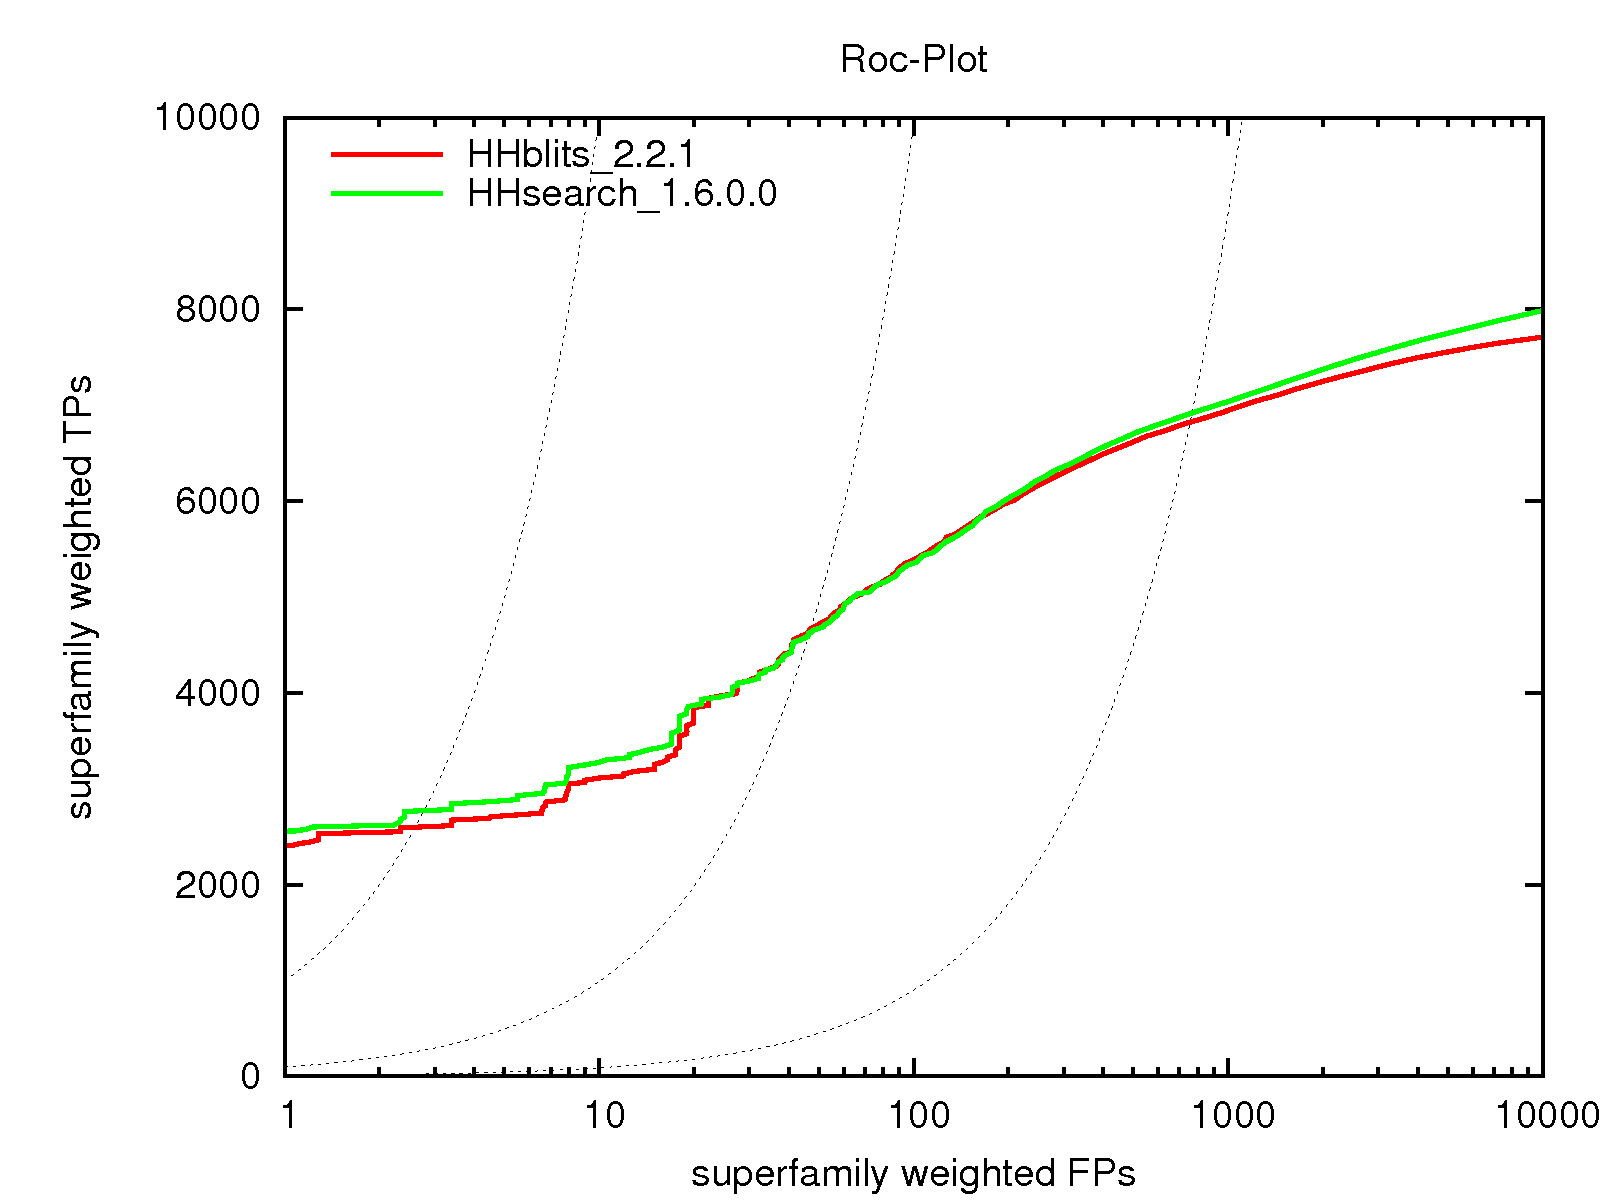
\includegraphics[width=0.5 \textwidth]{hhblits-hhsearch.png}
\caption{Benchmark of HHsearch and HHblits on a SCOP20 dataset.}
\label{fig:hhsearch_hhblits_bench}
\end{center}
\end{figure}

The hhblits tool can be used in much the same way as hhsearch. 
It takes the same input data and produces a results file in the same format as hhsearch.
Most of the hhsearch options also work for hhblits, which has
additional options associated with its extended functionality for iterative searches. 
Due to its fast prefilter, hhblits runs between 30 and 3000 times faster than HHsearch
at the cost of only a few percent lower sensitivity (Fig. \ref{fig:hhsearch_hhblits_bench}).
Whereas HHsearch only needs the file \verb`<dbname>_hhm_db`, HHblits needs the other files
belonging to the HH-suite database as well. 

The same search as above is performed here using hhblits instead of hhsearch:
\begin{verbatim}
$ hhblits  -cpu 4 -i data/query.a3m -d databases/scop70_1.75 -n 1
\end{verbatim}
Note that instead of specifying the up to eight database files explicitly, only their common prefix
is given (in this case \verb`databases/scop70_1.75`).

HHblits first scans the column state sequences in \verb`scop70_1.75.cs219` with its fast prefilter. HMMs whose column state sequences pass the prefilter are read from the packed file \verb`scop70_1.75_hhm_db` (using the index file \verb`scop70_1.75_hhm_db.index`) and are aligned to the query HMM generated from \verb`query.a3m` using the slow Viterbi HMM-HMM alignment algorithm. The search results are written to the default output file \verb`query.hhr`. The option \verb`-n 1` tells hhblits to perform a single search iteration. (The default is 2 iterations.)


\subsection{Generating a multiple sequence alignment using HHblits}\label{msa_hhblits}

To generate an MSA for a sequence or initial MSA in query.a3m, the database to be searched should cover the entire sequence space, such as uniprot20 or nr20. The option \verb`-oa3m <msa_file>` tells HHblits to generate an output MSA from the significant hits:
\begin{verbatim}
$ hhblits -cpu 4 -i data/query.seq -d databases/uniprot20 -oa3m query.a3m -n 1
\end{verbatim}

At the end of the search, HHblits reads from the packed database file containing the MSAs the sequences belonging to HMMs with E-value below the threshold. The E-value threshold for inclusion into the MSA can be specified using the \verb`-e <E-value>` option. After the search, \verb`query.a3m` will contain the MSA in A3M format. 

We could do a second search iteration, starting with the MSA from the previous search, to add more sequences. Since the MSA generated after the previous search contains more information than the single sequence in \verb`query.seq`, searching with this MSA will probably result in many more homologous database matches.
\begin{verbatim}
$ hhblits -cpu 4 -i query.a3m -d databases/uniprot20 -oa3m query.a3m -n 1
\end{verbatim}

Instead, we could start the search with \verb`query.seq` and directly perform two search iterations, by doing two search iterations using the option \verb`-n 2`:
\begin{verbatim}
$ hhblits -cpu 4 -i data/query.seq -d databases/uniprot20 -oa3m query.a3m -n 2 
\end{verbatim}

In practice, it is recommended to use between 1 and 4 iterations for building MSAs, depending on the trade-off between reliability and specificity on one side and sensitivity for remotely homologous sequences on the other side. The more search iterations are done, the higher will be the risk of non-homologous sequences or sequence segments entering the MSA and recruiting more of their kind in subsequent iterations. This is particularly problematic when searching with sequences containing short repeats, regions with amino acid compositional bias and, although less dramatic,  with multiple domains. Fortunately, this problem is much less pronounced in hhblits as compared to PSI-BLAST due to hhblits's lower number of iterations, its more robust Maximum Accuracy alignment algorithm, and the higher precision of its HMM-HMMs alignments. 

The parameter \verb`mact` (maximum accuracy threshold) lets you choose the trade-off between sensitivity and 
precision. With a low mact-value (e.g. \verb`-mact 0.01`) very sensitive, but not 
so precise alignments are generated, whereas a search with a high mact-value (e.g. \verb`-mact 0.9`) 
results in shorter but very precise alignments. The default value of mact in HHblits is $0.35$ 
(changed from 0.5 in the beta version). 

To avoid unnecessarily large and diverse MSAs, HHblits stops iterating when the diversity of the query MSA -- measured as number of effective sequences, see section \ref{aliformats} -- grows passed a threshold of 10.0. This threshold can be modified with the \verb`--neffmax <float>` option. See subsection \ref{hhmformat} for a description of how the number of effective sequences is calculated in HH-suite.

To avoid the final MSAs to grow unnecessarily large, by default the cluster MSAs are filtered with the option \verb`-diff 1000` prior to merging them with the query MSA. The \verb`-diff 1000` option selects the most representative sequences from an MSA such that every regions is covered by at least 1000 sequences. To turn off the filtering and obtain all sequences in the significantly similar uniprot20 clusters, use the \verb`-nodiff` option: 
\begin{verbatim}
$ hhblits -cpu 4 -i data/query.seq -d databases/uniprot20 -oa3m query.a3m -nodiff
\end{verbatim}

The A3M format uses small letters to mark inserts and capital letters to designate match and delete columns (see subsection \ref{aliformats}), allowing to omit gaps aligned to insert columns. The A3M format therefore uses much less space for large alignments than FASTA but looks misaligned to the human eye. Use the \verb`reformat.pl` script to reformat \verb`query.a3m` to other formats, e.g. for reformatting the MSA to Clustal and FASTA format, type

\begin{verbatim}
$ reformat.pl a3m clu query.a3m query.clu
$ reformat.pl a3m fas query.a3m query.fas
\end{verbatim}

Next, to add secondary structure information to the MSA we call the script \verb`addss.pl`. For \verb`addss.pl` to work, you have to make sure that the paths to BLAST and PSIPRED in the file \verb`scripts/HHPaths.pm` are correctly filled in. Then type
\begin{verbatim}
$ addss.pl query.a3m
\end{verbatim}
When the sequence has a SCOP or PDB identifier as first word in its name, the script tries to add the DSSP states as well. Open the \verb`query.a3m` file and check out the two lines that have been added to the MSA. Now you can generate a hidden Markov model (HMM) from this MSA:
\begin{verbatim}
$ hhmake -i query.a3m
\end{verbatim}
The default output file is \verb`query.hhm`. By default, the option \verb`-M first` will 
be used. This means that exactly those columns of 
the MSAs which contain a residue in the query sequence will be assigned to Match 
/ Delete states, the others will be assigned to Insert states. (The query sequence is 
the first sequence not containing secondary structure information.) Alternatively, you 
may want to apply the 50\%-gap rule by typing \verb`-M 50`, which assigns only those columns 
to Insert states which contain more than 50\% gaps. The \verb`-M first` option makes sense 
if your alignment can best be viewed as a seed sequence plus aligned homologs to 
reinforce it with evolutionary information. This is the case in the SCOP and PDB 
versions of our HMM databases, since here MSAs are built around a single seed 
sequence (the one with known structure). On the contrary, when your alignment 
represents an entire family of homologs and no sequence in particular, it is best to 
use the 50\% gap rule. This is the case for Pfam or SMART MSAs, for instance. 
Despite its simplicity, the 50\% gap rule has been shown to perform well in practice.

When calling \verb`hhmake`, you may also apply several filters, such as maximum pairwise 
sequence identity (\verb`-id <int>`), minimum sequence identity with query sequence 
(\verb`-qid <int>`), or minimum coverage with query (\verb`-cov <int>`). But beware 
of reducing the diversity of your MSAs too much, as this will lower the sensitivity to
detect remote homologs.

Previous versions of HH-suite (the 'HHsearch package') included a perl script \verb`buildali.pl` to build MSAs for a query sequence using PSI-BLAST as its search engine. Because HHblits performs better than PSI-BLAST in all aspects that we have tested, we decided to remove this script from HH-suite. It can still be downloaded as part of HHsearch version 1.5.0.


\subsection{Building customized databases} \label{building_dbs}

It is simple to build custom HH-suite databases using the same tools we use to build the standard HH-suite databases (except uniprot20 and nr20). An example application is to search for homologs among all proteins of an organism. To build your own HH-suite database from a set of sequences, you first need to generate an MSA with predicted secondary structure for every sequence in the set. This can conveniently be done using the script \verb`multithread.pl` in the HH-suite. This script runs a command for many files in parallel, distributing the individual jobs to multiple cores on your server, one file per thread. This will shorten the run-time roughly by the number of cores. 

To run \verb`multithread.pl`, you need first to have each sequences in a separate FASTA-formatted file. If your sequences are contained in a single multiple-sequence FASTA file \verb`<dbseqs.fas>`, first split them up into multiple single-sequence files using \verb`splitfasta.pl`:
\begin{verbatim}
$ mkdir dbs/scop70_1.75; cd dbs/scop70_1.75
$ splitfasta.pl <dbseqs.fas> 
\end{verbatim}
Now, to build an MSA with HHblits for each sequence \verb`dbs/scop70_1.75/*.seq`, run\\[-1mm]

\verb`$ multithread.pl 'dbs/scop70_1.75/*.seq' `\\
\verb`                       'hhblits -i $file -d databases/uniprot20 -oa3m $name.a3m'`\\[-1mm]

The first argument is the file globbing expression (protected from the shell by quotes), which selects the files with which to run the command. The command is given as second argument within quotes. In this command, the string \verb`$file` is replaced by the actual, globbed file. You might also want to pipe the stdout and stderr streams of the command into a log-file:\\
\verb`'hhblits -i $file -d databases/uniprot20 1> stdout.log 2>stderr.log'`. 
The MSAs are written to the file \verb`$name.a3m`. Here, \verb`$name` stands for the globbed file name without its extension. The number of threads to launch can be specified with option \verb`-cpu <int>` (default value is 8). To be sure that everything went smoothly, check that the number of \verb`*.a3m` files is the same as the number of \verb`*.seq` files, and browse the file \verb`'stderr.log'` for error messages. The number of HHblits search iterations and the HMM inclusion E-value threshold for hhblits can be changed from their default values (2 and 0.01, respectively) using the \verb`'-n <int>'` and \verb`'-e <float>'` options.

Now, add PSIPRED-predicted secondary structure to all MSAs:
\begin{verbatim}
$ multithread.pl 'dbs/scop70_1.75/*.a3m' 'addss.pl $file' -cpu 16 
\end{verbatim}
Again, piping stdout and stderr into log files and inspecting the warnings and errors is recommended. 

An HH-suite database consists of eight files, as described in subsection \ref{hhblits_dbs}. These files can be generated by a single call to \verb`hhblitsdb.pl`:
\begin{verbatim}
$ hhblitsdb.pl -o databases/scop70_1.75 -ia3m dbs/scop70_1.75/ -cpu 16
\end{verbatim}
In order to build the file containing the column state sequence for prefiltering, \verb`hhblitsdb.pl` will generate a column state sequence for each A3M-formatted MSA in the directory given by the \verb`-ia3m` option. As this can take some time, the script calls \verb`multithread.pl` to distribute the jobs to multiple cores. The script also needs to generate an HHM files for each MSA file, for which again \verb`multithread.pl` is called. In the end, the \verb`ffindex` utility generates the packed files containing the A3M MSAs and HHM models with corresponding index files. The script will report the number of files of each category (column-state, A3M, HHM) and warn if the numbers differ. The option \verb`-log err.log` pipes the stderr stream of each command executed into a log file. As with all perl scripts in the HH-suite, a list of additional options can be retrieved by calling the scripts without parameters.

Alternatively, if you have a set of HHM or HMMER model files but no MSA files, for example for Pfam, you can build an HH-suite database with the command
\begin{verbatim}
$ hhblitsdb.pl -o databases/pfamA_25 -ihhm dbs/pfamA_25/ -hhmext hmm -cpu 16
\end{verbatim}
The script will then build the column state sequences from the HMMER files in the directory given by the \verb`-ihhm` option. It will then generate the five database files that are needed by \verb`hhblits` for non-iterative searches throug the database. (The three files referring to the A3M MSAs cannot be built since no MSAs were supplied. However, these file are only needed to build output MSAs with the -oa3m option or to build a query MSA for a second search iteration. They are dispensable for non-iterative searches.)

Please note that HHblits and HHsearch lose quite a lot of performance when using HMMER-formatted HMMs instead of HH-suite-formatted ones. We therefore strongly recommend to build HH-suite formatted HMMs directly from the MSAs if possible. (Pfam MSAs can be retrieved from our ftp site.)


\subsubsection*{Old-style HHsearch databases}

An old-style HHsearch database consists simply of concatenated hhm files. Start from the a3m files including predicted secondary structure, generated as described above. Then generate the \verb`hhm` files using \verb`multithread.pl`:
\begin{verbatim}
$ multithread.pl 'dbs/scop70_1.75/*.a3m' 'hhmake -i $file' -cpu 8 
\end{verbatim}
The \verb`hhm` files will have the same name but with a different extension as their \verb`a3m` files. You 
can then concatenate your individual HMMs into your database:
\begin{verbatim}
$ cat *.hhm > scop70_1.75.hhm
\end{verbatim}
or, if the maximum command line buffer size is exceeded, 
\begin{verbatim}
$ find $tmpdir -name '*.seq219' -exec cat '{}' + >> scop70_1.75.hhm
\end{verbatim}



\section{Frequently asked questions}

\subsection{How do I report a bug?}
If you find a bug, PLEASE tell us about it. But first, make sure the problem is not due to wrong usage or wrong file formats. This requires having read the relevant sections of the user guide. (Sorry!) Check for possible warnings. Rerun the command with verbose option \verb`-v 3` or \verb`-v 4` to see if you can find where things go awry. If the problem persists, we will need everything to reproduce the bug on our machines. Please send us (1) the input file, (2) the database name and version, or, if it is not a standard database, the link to your ftp server to download the database files, (3) the output files, (4) the command and its screen output, (5) the operating system and CPU on which the bug occurred. Under Linux, please send us the output of 
\small
\begin{verbatim}
$ echo $HHLIB $PATH; uname -a; lsb_release -a; head -n 25 /proc/cpuinfo; ulimit -a; free
\end{verbatim}
\normalsize
Thanks a lot!

\subsection{What is HMM-HMM comparison and why is it so powerful?}
When searching for remote homologs, it is wise to make use of as much information about the query and database proteins as possible in order to better distinguish true from false positives and to produce optimal alignments. This is the reason why sequence-sequence comparison is inferior to profile-sequence comparison. Sequence profiles contain for each column of a multiple alignment the frequencies of the 20 amino acids. They therefore contain detailed information about the conservation of each residue position, i.e. how important each position is for defining other members of the protein family, and about the preferred amino acids. Profile Hidden Markov Models (HMMs) are similar to simple sequence profiles, but in addition to the amino acid frequencies in the columns of a multiple sequence alignment they contain information about the frequency of inserts and deletions at each column. Using profile HMMs in place of simple sequence profiles should therefore further improve sensitivity. Using HMMs both on the query and the database side greatly enhances the sensitivity/selectivity and alignment quality over sequence-profile based methods such as PSI-BLAST. HHsearch is the first software to employ HMM-HMM comparison and HHblits is the first profile-profile comparison method that is fast enough to do iterative searches to build MSAs. 

\subsection{When can the HH-suite be useful for me?}
Sequence search methods such as BLAST, FASTA, or PSI-BLAST are of prime importance for biological research because functional information of a protein or gene can be inferred from homologous proteins or genes identified in a sequence search. But quite often no significant relationship to a protein of known function can be established. This is certainly the case for the most interesting group of proteins, those for which no ortholog has yet been studied. In cases where conventional sequence search methods fail, HHblits and HHsearch quite often allow to make inferences from more remotely homologous relationships. HHblits builds better MSAs, with which more remote homologs can then be found using HHsearch or HHblits, e.g. by searching the PDB or domain databases such as Pfam. If the relationship is so remote that no common function can be assumed, one can often still derive hypotheses about possible mechanisms, active site positions and residues, or the class of substrate bound \cite{Todd:2001, Pawlowski:2000}. When a homologous protein with known structure can be identified, its stucture can be used as a template to model the 3D structure of the protein of interest \cite{Rychlewski:1998}, since even protein domains that shared a common ancestor some 3 billion years ago mostly have similar 3D structures \cite{Kinch:2002,Soding:2006a,Alva:2010}. The 3D model may then help to generate hypotheses to guide experiments. 

\subsection{What does homology mean and why is it important?}
Two protein sequences are homologous to each other if they descended from a common ancestor sequence. Generally, homologous proteins (or protein fragments) have similar structure because structures diverge much more slowly than their sequences \cite{Chothia:1986}. Depending on the degree of divergence between the sequences, the proteins may also have similar cellular functions, ligands, protein interaction partners, or enzymatic mechanisms \cite{Todd:2001}. On the contrary, proteins that have a similar structure by convergence (i.e. by chance) are said to be analogous. They don't generally share similar functions or biochemical mechanisms and are therefore much less helpful for making inferences. HHsearch and HHblits are tools for homology detection and as such do not normally detect analogous relationships \cite{Alva:2010,Remmert:2010}.


\subsection{How can I verify if a database match is homologous?}
Here is a list of things to check if a database match really is at least locally homologous.
 
{\bf Check probability and E-value}:
HHsearch and HHblits can detect homologous relationships far beyond the twilight zone, i.e. below 20\% sequence identity. Sequence identity is therefore not an appropriate measure of relatedness anymore. The estimated probability of the template to be (at least partly) homologous to your query sequence is the most important criterion to decide whether a template HMM is actually homologous or just a high-scoring chance hit. When it is larger than 95\%, say, the homology is nearly certain. Roughly speaking, one should give a hit serious consideration (i.e. check the other points in this list) whenever (1) the hit has $>50\%$ probability, or (2) it has $>30\%$ probability and is among the top three hits. The E-value is an alternative measure of statistical significance. It tells you how many chance hits with a score better than this would be expected if the database contained only hits unrelated to the query. At E-values below one, matches start to get marginally significant. Contrary to the probability, when calculating the E-value HHsearch and HHblits do not take into account the secondary structure similarity. Therefore, the probability is a more sensitive measure than the E-value.

{\bf Check if homology is biologically suggestive or at least reasonable}:
Does the database hit have a function you would expect also for your query? Does it come from an organism that is likely to contain a homolog of your query protein?

{\bf Check secondary structure similarity}:
If the secondary structure of query and template is very different or you can't see how they could fit together in 3D, then this is a reason to distrust the hit. Note however that if the query alignment contains only a single sequence, the secondary structure prediction is quite unreliable and confidence values are overestimated.

{\bf Check relationship among top hits}: 
If several of the top hits are homologous to each other, (e.g. when they are members of the same SCOP superfamily), then this will considerably reduce the chances of all of them being chance hits, especially if these related hits are themselves not very similar to each other. Searching the SCOP database is very useful precisely for this reason, since the SCOP family identifier (e.g. a.118.8.2) allows to tell immediately if two templates are likely homologs.

{\bf Check for possible conserved motifs}:
Most homologous pairs of alignments will have at least one (semi-)conserved motif in common. You can identify such putative (semi-)conserved motifs by the agglomeration of three or more well-matching columns (marked with a '\verb`|`' sign between the aligned HMMs) occurring within a few residues, as well as by matching consensus sequences. Some false positive hits have decent scores due to a similar amino acid composition of the template. In these cases, the alignments tend to be long and to lack conserved motifs.

{\bf Check residues and role of conserved motifs}: 
If you can identify possible conserved motifs, are the corresponding conserved template residues involved in binding or enzymatic function?

{\bf Check query and template alignments}: 
A corrupted query or template alignment is the main source of high-scoring false positives. The two most common sources of corruption in an alignment are (1) non-homologous sequences, especially repetitive or low-complexity sequences in the alignment, and (2) non-homologous fragments at the ends of the aligned database sequences. Check the query and template MSAs in an alignment viewer such as Jalview or ALNEDIT.

{\bf Realign with other parameters}: 
change the alignment parameters. Choose global instead of local mode, for instance, if you expect your query to be globally homologous to the putative homolog. Try to improve the probability by changing the values for minimum coverage or minimum sequence identity. You can also run the query HMM against other databases.

{\bf Build the query and/or database MSAs more aggressively}:
If your query (or template) MSA is not diverse enough, you could increase sensitivity substantially by trying to include more remotely homologous sequences into the MSA. Try using our HHsenser web server at \url{http://toolkit.tuebingen.mpg.de/hhsenser} \cite{Soding:2006b}. Check the HHsenser alignment manually using an alignment editor. Have non-homologous sequences or sequence segments been accidentally included? You can also try to build a more diverse MSA manually: Inspect the HHblits results after the first iteration and consider including hits above the E-value inclusion threshold of 0.001, based on biological plausibility, relatedness of the organism, a reasonable looking alignment, or just guessing. Then start the second HHblits search iteration HHblits with this manually enriched alignment. 

{\bf Try out other tools}:
Try other tools (e.g. for profile-profil comparison) and servers for remote homology detection and structure prediction. 
A list of servers can be found in \cite{Mariani:2011} and \cite{Battey:2007}.

{\bf Verify predictions experimentally}: 
The ultimate confirmation of a homologous relationship or structural model is, of course, the experimental verification of some of its key predictions, such as validating the binding to certain ligands by binding assays, measuring biochemical activity, or comparing the knock-out phenotype with the one obtained when the putative functional residues are mutated.


\subsection{What does the maximum accuracy alignment algorithm do?} \label{MAC}
HHblits and HHsearch use a better alignment algorithm than the quick and 
standard Viterbi method to generate the final HMM-HMM alignments. Both realign
all displayed alignments in a second stage using the more accurate Maximum Accuracy 
(MAC) algorithm \cite{Durbin:2008,Biegert:2008}. The Viterbi algorithm is employed 
for searching and ranking the matches. The realignment step is parallelized 
(\verb`-cpu <int>`) and typically takes a few seconds only.    

Please note: Using different alignment algorithms for scoring and aligning has the 
disadvantage that the pairwise alignments that are displayed are not always very similar to 
those that are used to calculate the scores. This can lead to confusing results 
where alignments of only one or a few residues length may have obtained significant
E-values. In such cases, run the search again with the \verb`-norealign` option, which will 
skip the MAC-realignment step. This will allow you to check if the Viterbi alignments 
are valid at all, which they will probably not be. The length of the MAC alignments 
can therefore give you additional information to decide if a match is valid. In order
to avoid confusion for users of our HHpred server \cite{Soding:2005b, Hildebrand:2009}, 
the \verb`-norealign` option is the default there, whereas for you pros who dare to use 
the command line package, realigning is done by default.

The posterior probability threshold is controlled with the -mact [0,1[ option. 
This parameter controls the alignment algorithm's greediness. More precisely, the 
MAC algorithm finds the alignment that maximizes the sum of posterior probabilities 
minus mact for each aligned pair. Global alignments are generated with -mact 0, 
whereas -mact 0.5 will produce quite conservative local alignments. 

The -global and -local options now refer to both the Viterbi search stage as 
well as the MAC realignment stage. With -global (-local), the posterior probability 
matrix will be calculated for global (local) alignment. When -global is used in 
conjunction with -realign, the mact parameter is automatically set to 0 in order to 
produce global alignments. In other words, both following two commands will give 
global alignments:
\begin{verbatim}
$ hhsearch -i <query> -d <db.hhm> -realign -mact 0
$ hhsearch -i <query> -d <db.hhm> -realign -global
\end{verbatim}

The first version uses \emph{local} Viterbi to search and then uses MAC to realign the 
proteins globally (since mact is 0) on a \emph{local} posterior probability matrix. The 
second version uses \emph{global} Viterbi to search and then realigns globally (since mact 
is automatically set to 0) on a \emph{global} posterior matrix. To detect and align remote 
homologs, for which sometimes only parts of the sequence are conserved, the first 
version is clearly better. It is also more robust. If you expect to find globally 
alignable sequence homologs, the second option might be preferable. In that case, 
it is recommended to run both versions and compare the results. 

\subsection{How is the MSA diversity NEFF (the number of effective sequences) calculated?}
The number of effective sequences of the full alignment, which appears as NEFF in the header of each hhm file, is the average of local values \verb`Neff_M(i)` over all alignment positions $i$. The values \verb`Neff_M(i)` are given in the main model section of the hhm model files (subsection \ref{hmmformat}). They quantify the \emph{local} diversity of the alignment in a region around position $i$. More precisely, \verb`Neff_M(i)` measures the diversity of subalignment $Ali_M(i)$ that contains all sequences that have a residue at column $i$ of the full alignment. The subalignment contains all columns for which at least 90\% of these sequences have no end gap. End gaps are gaps to the left of the first residue or to the right of the last residue. The latter condition ensures that the sequences in the subalignment $Ali_M(i)$ cover most of the columns in it. The number of effective sequences in the subalignment $Ali_M(i)$ is exp of the average sequence entropy over all columns of the subalignment. Hence, \verb`Neff_M` is bounded by 0 from below and 20 from above. In practice, it is bounded by the entropy of a column with background amino acid distribution $f_a$: $N_{eff} < \sum_{a=1}^{20} f_a \log f_a \approx 16$. Similarly, \verb`Neff_I(i)` gives the diversity of the subalignment $Ali_I(i)$ of all sequences that have an insert at position $i$, and \verb`Neff_D(i)` refers to the diversity of subaligment $Ali_D(i)$ of all sequences that have a Delete (a gap) at position $i$ of the full alignment. 



\subsection{More frequently asked questions}

{\bf How can I retrieve individual database A3M or HHM files in my HH-suite database?}
For reasons of efficiency, the MSA A3M and HHM model files are packed into two files, \verb`<db>_a3m_db` and \verb`<db>_hhm_db`, each with its own index file. The contained files are easy to extract from the packed files. For example, to dump \verb`d1aa7a_.a3m` in \verb`scop70` to standard output, type 
\begin{verbatim}
$ ffindex_get scop70_a3m_db  scop70_a3m_db.index d1aa7a_.a3m
\end{verbatim}
You may write the extracted file to a separate file by appending \verb`'> d1aa7a_.a3m'` to the above command.


{\bf Do HHsearch and HHblits work fine with multi-domain sequences?}
HHblits and HHsearch have been designed to work with multi-domain queries. However, the chances for false positives entering the query alginment during the HHblits iterations is greater for multi-domain proteins. For long sequences, it may therefore be of advantage to first search the PDB or the SCOP domain database and then to cut the query sequence into smaller parts on the basis of the identified structural domains. Pfam or CDD are - in our opinion - not suitable to determine domain boundaries.

{\bf Don't I need to calibrate my query or database HMMs anymore?}
No. If you don't specify otherwise, the two parameters of the extreme-value distribution for the query are estimated by a neural network from the lengths and diversities ($N_\mathrm{eff}$)) of query and database HMMs that was trained on a large set of example queries-template pairs, in an approach simlar to the one used in \cite{Sadreyev:2008}. However, the old calibration is still available as an option in HHsearch.

{\bf How can I build my own UniProt database for HHblits?}
The procedure to cluster the nr or UniProt databases is more complicated than building a database for a genome or for the sequences in the pdb. As its first step it involves clustering these huge databases down to 20\%-30\% sequence identity. The clustering is done in our lab using a new method, kClust (Hauser M, Mayer CE, and Soeding J., to be published), available und GPL at \url{ftp://ftp://toolkit.lmb.uni-muenchen.de/kClust/}. We will add all scripts to build these HH-suite databases to the HH-suite in due time. These scripts generate A3M files, HHM files, and consensus sequences. Because of the large number of files to generate, these scripts need to be run on a computer cluster and this will require considerable computer savvyness. 

{\bf Will you offer an HH-suite database that includes environmental sequences?}
We have not seen significant improvements in remote homology detection through inclusion of environmental sequences. A problem with these sequences is their low quality, in particular chimeric sequences from wrong assemblies. This can lead to corrupted profiles in iterative searches. We therefore have no immediate plans to provide a UniProt+env or nr+env for hhblits. If you think you really need the env sequences, you have to use our old \verb`buildali.pl` script or PSI-BLAST for the time being. An alternative is to use kClust to cluster the database yourself. See the previous question.

{\bf Why do I sometimes get the same database hit twice with different probabilities? Is this a bug?} Each line in the summary hit list refers to an alignment with an HMM in the database, not to the database HMM itself. Sometimes, alternative (suboptimal) alignments covering a different part of either the query or the database HMM may appear in the hit list. Usually, both the optimal and the alternative alignments are correct, in particular when the query or the database HMMs represent repeat proteins. 

{\bf How do I reconcile overlapping and conflicting domain predictions, for example domain A predicted from residues 2-50 with 98\% probability and domain B from 2-200 with 95\% probability?} The probability that a pair of residues is correctly aligned is the product of the probability for the database match to be homologous (given by the values in the \verb`Probab` column of the hit list) times the posterior probability of the residue pair to be correctly aligned given the database match is correct in the first place. The posterior probabilities are specified by the confidence numbers in the last line of the alignment blocks (0 corresponds approximately to 0-10\%, 9 to 90-100\%). Therefore, an obvious solution is to prune the alignments in the overlapping region such that the sum of total probabilities is maximized. There is no script yet that does this automatically.

{\bf Why do I get different results when I search with the same query through the same database using hhblits and hhsearch?} There are two reasons. First, some hits that hhsearch shows might not have passed the prefilter in hhblits. The option \verb`-prepre_smax_thresh <bits>` lets you modify the minimum score threshold of the first, gapless alignment prefilter (default is 10 bits). Option \verb`-pre_evalue_thresh <E-value>` sets the maximum E-value threshold for the second, gapped alignment prefilter (default is 1000). Second, while the probabilities and P-values of hhblits and hhsearch should be the identical for the same matches, the E-values are only similar. The reason is that hhblits heuristically combines the E-values of the second prefilter with the E-values from the full HMM-HMM Viterbi alignment into total E-values \cite{Remmert:2011}. These E-values are slightly better in distinguishing true from false hits, because they combine the partly independent information from two comparisons.

{\bf I want to build a phylogenetic tree for HMMs. Which measure of similarity should I use?}
I would use something like the raw score per alignment length. (You might also add the secondary structure score to the raw score.) Probabilities, E-values, and P-values are useful for deciding whether a match is a reliable homolog or not. They are not suitable for measuring similarities, because they strongly depend on the length of the alignment, roughly like $\mathrm{P-value} \propto \exp(\lambda \times \mathrm{average\_similarity} \times \mathrm{length})$, with some constant $\lambda$ or order 1. The probability has an even more complex dependence on length. The Similarity given above the alignment blocks does not capture the evolutionary information contained in the MSAs (see subsection \ref{aliblocksformat}). One note of caution: Large, diverse MSAs are usually more sensitive to find homologs than narrower ones. Therefore, I would limit the diversity of all HMMs to some reasonable number (perhaps around 5 or 7, depending on how far diverged your HMMs are). This filtering can be done using \verb`$ hhfilter -i <MSA.a3m> -o <MSA_filt.a3m> -neff 5`, for example. 

{\bf Should I use the \verb`-global` option to build MSAs for an HH-suite database if I am intersted in global alignments to these database HMMs?}
Never use \verb`-global` when building MSAs by iterative searches with HHblits. Remember that global alignments are very greedy alignments, where alignments stretch to the ends of either query of database HMM, no matter what. Global alignments will therefore often lead to non-homologous segments getting included in the MSA, which is catastrophic, as these false segments will lead to many false positive matches when searching with this MSA. But you may use \verb`-global` when searching (with a single iteration) for global matches of your query HMMs through your customized HH-suite database, for example.

{\bf How many iterations of hhblits should I use to search my customized genome database?} One iteration! Doing more than one search iterations in general only makes sense in order to build up a diverse MSA of homologous sequences by searching through the uniprot20 or nr20 databases. 




\section{HHsearch/HHblits output: hit list and pairwise alignments}\label{outformat}

\subsection{Summary hit list}

Let's do a search with the human PIP49/FAM69B protein, for which we generated an MSA in \verb`query.a3m` with two iterations of HHblits in subsection \ref{msa_hhblits}:

\scriptsize
\begin{verbatim}
Search results will be written to query.hhr
query.a3m is in A2M, A3M or FASTA format
Read query.a3m with 272 sequences
Alignment in query.a3m contains 431 match states
149 out of 270 sequences passed filter (up to 91% position-dependent max pairwise sequence identity)
Effective number of sequences exp(entropy) = 5.2 
.................................................. 1000 HMMs searched
.................................................. 2000 HMMs searched
.................................................. 3000 HMMs searched
.................................................. 4000 HMMs searched
.................................................. 5000 HMMs searched
.................................................. 6000 HMMs searched
.................................................. 7000 HMMs searched
.................................................. 8000 HMMs searched
.................................................. 9000 HMMs searched
.................................................. 10000 HMMs searched
.................................................. 11000 HMMs searched
.................................................. 12000 HMMs searched
.................................................. 13000 HMMs searched
....................................
Realigning 183 query-template alignments with maximum accuracy (MAC) algorithm ...

Query         sp|Q5VUD6|FA69B_HUMAN Protein FAM69B OS=Homo sapiens GN=FAM69B PE=2 SV=3
Match_columns 431
No_of_seqs    149 out of 272
Neff          5.2 
Searched_HMMs 13730
Date          Wed Jan  4 17:44:24 2012
Command       /cluster/user/soeding/hh/src/hhsearch -i query.a3m -d /cluster/user/soeding/databases/scop.hhm -cpu 18 

 No Hit                             Prob E-value P-value  Score    SS Cols Query HMM  Template HMM
  1 d1qpca_ d.144.1.7 (A:) Lymphoc  99.7 4.5E-17 3.2E-21  154.3  10.2   99  203-320    56-157 (272)
  2 d1jpaa_ d.144.1.7 (A:) ephb2 r  99.7 4.3E-17 3.1E-21  156.8   8.8   99  203-321    75-177 (299)
  3 d1uwha_ d.144.1.7 (A:) B-Raf k  99.7 5.1E-17 3.7E-21  154.8   7.7  100  203-322    52-154 (276)
  4 d1opja_ d.144.1.7 (A:) Abelson  99.7 6.2E-17 4.5E-21  154.8   8.3  100  203-321    61-164 (287)
  5 d1mp8a_ d.144.1.7 (A:) Focal a  99.6 9.9E-17 7.2E-21  151.3   8.6  100  203-322    56-158 (273)
  6 d1sm2a_ d.144.1.7 (A:) Tyrosin  99.6 1.2E-16 8.8E-21  150.3   8.8   99  203-321    48-150 (263)
  7 d1u59a_ d.144.1.7 (A:) Tyrosin  99.6 2.4E-16 1.7E-20  150.9   9.5   99  203-321    57-158 (285)
  8 d1xbba_ d.144.1.7 (A:) Tyrosin  99.6 2.2E-16 1.6E-20  150.2   8.6   97  203-320    56-155 (277)
  9 d1vjya_ d.144.1.7 (A:) Type I   99.6 2.6E-16 1.9E-20  151.3   8.8   98  204-320    46-156 (303)
 10 d1mqba_ d.144.1.7 (A:) epha2 r  99.6 4.4E-16 3.2E-20  148.0   8.7  193  203-422    57-272 (283)
...
 64 d1j7la_ d.144.1.6 (A:) Type II  97.3 0.00014   1E-08   65.0   6.3   33  292-324   184-216 (263)
 65 d1nd4a_ d.144.1.6 (A:) Aminogl  96.7  0.0012 8.5E-08   58.5   6.6   31  292-322   176-206 (255)
 66 d1nw1a_ d.144.1.8 (A:) Choline  96.6  0.0011 7.8E-08   63.9   5.8   37  203-239    92-128 (395)
 67 d2pula1 d.144.1.6 (A:5-396) Me  95.6  0.0071 5.2E-07   58.3   6.4   32  290-322   222-253 (392)
 68 d1a4pa_ a.39.1.2 (A:) Calcycli  91.7    0.12 8.9E-06   40.0   5.4   62  140-202    18-80  (92)
 69 d1ksoa_ a.39.1.2 (A:) Calcycli  91.2    0.17 1.2E-05   39.5   5.8   56  147-203    28-83  (93)
 70 d1e8aa_ a.39.1.2 (A:) Calcycli  90.5    0.23 1.7E-05   38.3   6.0   56  147-203    27-82  (87)
...
175 d1qxpa2 a.39.1.8 (A:515-702) C  23.7      29  0.0021   28.8   3.8   49  137-197    69-118 (188)
176 d1tuza_ a.39.1.7 (A:) Diacylgl  23.5      55   0.004   25.3   5.3   55  143-201    44-106 (118)
177 d1ggwa_ a.39.1.5 (A:) Cdc4p {F  23.1      26  0.0019   27.0   3.2   66  129-197    35-101 (140)
178 d1topa_ a.39.1.5 (A:) Troponin  22.8      72  0.0052   24.5   6.0   58  140-199    65-123 (162)
179 d1otfa_ d.80.1.1 (A:) 4-oxaloc  22.5      66  0.0048   21.5   5.0   40  267-306    12-53  (59)
180 d1oqpa_ a.39.1.5 (A:) Caltract  22.2      32  0.0023   24.0   3.2   32  165-197     3-34  (77)
181 d1df0a1 a.39.1.8 (A:515-700) C  21.7      43  0.0032   27.0   4.5   51  137-199    67-118 (186)
182 d1zfsa1 a.39.1.2 (A:1-93) Calc  21.1      41   0.003   24.6   3.8   30  170-199     8-38  (93)
183 d1snla_ a.39.1.7 (A:) Nucleobi  20.9      23  0.0016   26.2   2.2   24  174-197    18-41  (99)

Done
\end{verbatim}
\normalsize
 
The summary hit list that is written to the screen shows the best hits from the 
database, ordered by the probability of being a true positive (column 4: 'Prob'). 
The meaning of the columns is the following:
\vspace{5mm}

\renewcommand{\arraystretch}{1.2}

\begin{description}
\item{\verb`No`}: the index of the datbase match.

\item{\verb`Hit`}: the first 30 characters of the name line.

\item{\verb`Prob`}: the Probability of template to be a true positive.
For the probability of being a true positive, the secondary structure score 
in column \verb`SS` is taken into account, together with the raw score incolumn \verb`Score`. 
True positives are defined to be either globally homologous or they are at least 
homologous in parts, and thereby locally similar in structure. More precisely, 
the latter criterion demands that the MAXSUB score between query and hit is at 
least 0.1. In almost all cases the structural similarity will we be due to a global
OR LOCAL homology between query and template.

\item{\verb`E-value`}:
The E-value gives the average number of false positives ('wrong hits') with a score 
better than the one for the template when scanning the database. It is a measure of 
reliability: E-values near to 0 signify a very reliable hit, an E-value of 10 means 
about 10 wrong hits are expected to be found in the database with a score at least 
this good. Note that E-value and P-value are calculated without taking the secondary 
structure into account!


\item{\verb`P-value`}: 
The P-value is the E-value divided by the number of sequences in the database.
It is the probability that in a \emph{pairwise} comparison a wrong hit will score at least 
this good.

\item{\verb`Score`}: the raw score is what comes out of the (Viterbi) HMM-HMM alignment excluding
the secondary structure score. Informally speaking, it is the sum over the similarities 
of aligned profile colmuns minus the gap penalties. 

\item{\verb`SS`}: the secondary structure score.
This score tells you how well the PSIPRED-predicted (3-state) or actual DSSP-determined 
(8-state) secondary structure sequences agree with each other. PSIPRED confidence 
values are used in the scoring, low confidences getting less statistical weight.

\item{\verb`Cols`}: the number of aligned Match columns in the HMM-HMM alignment.

\item{\verb`Query HMM`}: the range of aligned match states from the query HMM.

\item{\verb`Template HMM`}: the range of aligned match states from the database/template HMM and, 
in parenthesis, the number of match states in the database HMM.

\end{description}



\subsection{HMM-HMM pairwise alignments}\label{aliblocksformat}

The output file d1bpya1.hhr contains the same hit list plus the pairwise HMM alignments. One example is give here:

\scriptsize
\begin{verbatim}
No 68 
>d1a4pa_ a.39.1.2 (A:) Calcyclin (S100) {Human (Homo sapiens), P11 s100a10, calpactin [TaxId: 9606]}
Probab=91.65  E-value=0.12  Score=40.00  Aligned_cols=62  Identities=16%  Similarity=0.149  Sum_probs=42.0

Q ss_pred             ccCCCCCCcHHHHHHHHHHHHHhhcccCccHHHHHHHHHhhhhccCCCCcCHHHHHHH-HHHHH
Q sp|Q5VUD6|FA69  140 FDKPTRGTSIKEFREMTLSFLKANLGDLPSLPALVGQVLLMADFNKDNRVSLAEAKSV-WALLQ  202 (431)
Q Consensus       140 ~d~p~~g~s~~eF~emv~~~i~~~lg~~~~l~~L~~~~~~~~d~nk~g~vs~~e~~sl-waLlq  202 (431)
                      ||+..-..|.+||.+++.......++.+.+ ...+..++..+|.|+||+|++.|...+ ..|..
T Consensus        18 yd~ddG~is~~El~~~l~~~~~~~~~~~~~-~~~v~~~~~~~D~n~DG~I~F~EF~~li~~l~~   80 (92)
T d1a4pa_          18 FAGDKGYLTKEDLRVLMEKEFPGFLENQKD-PLAVDKIMKDLDQCRDGKVGFQSFFSLIAGLTI   80 (92)
T ss_dssp             HHGGGCSBCHHHHHHHHHHHCHHHHHHSCC-TTHHHHHHHHHCTTSSSCBCHHHHHHHHHHHHH
T ss_pred             HcCCCCEEcHHHHHHHHHHhccccccccCC-HHHHHHHHHHHhCCCCCCCcHHHHHHHHHHHHH
Confidence            444433449999999998876655554332 234566677899999999999997544 44443
\end{verbatim}\normalsize

This alignment shows an EF hand embedded in a kinase domain in PIP49/FAM69B. The first line, 
which begins with with a ``\verb`>`'', contains the name and description line of the template/database 
HMM. (We use ``template HMM'' and ``matched database HMM'' synonymously.) 
The next line summarizes the main statistics for the alignment: The probability for the query and 
template HMMs to be homologous (\verb`Probab`), the \verb`E-value`, the raw \verb`Score`, and the 
number of aligned columns are repeated from the summary hit list. The \verb`Identities` give the percentage
of aligned residue pairs of the query and the template master sequences that are identical. 
The \verb`Similarity` is the arithmetic mean of the substitution scores between the aligned residue
pairs from the query and template master sequences. The substitution matrix is the same as the
one used to calculate the pseudocounts for the database HMMs, by default the Gonnet matrix. 
(The matrix can be changed with the \verb`-Blosom<XX>` option.) 

The \verb`Sum_probs` value is the sum over the posterior probabilities of all aligned pairs 
of match states. These probabilities are calculated by the Forward-Backward algorithm. 
(They are used by the maximum accuracy algorithm 
which computes the final alignments.) When the template HMM has secondary structure annotation from
DSSP, the \verb`sum_probs` value runs only over aligned pairs for which the template has a 
valid DSSP state, not a \verb`-` sign. A  \verb`-` would indicate that the structural coordinates of
that residue are missing in the template. For homology modelling, this special treatment of templates 
with known structure makes \verb`sum_probs` a useful feature to use for ranking templates.



The pairwise alignment consists of one or more blocks with the following lines:

\small
\begin{verbatim}
Q ss_dssp:      the query secondary structure as determined by DSSP (when available)
Q ss_pred:      the query secondary structure as predicted by PSIPRED (when available)
Q <Q_name>:     the query master sequence
Q Consensus:    the query alignment consensus sequence
\end{verbatim}\normalsize

The predicted secondary structure states are shown in capital letters if the PSIPRED
confidence value is between 0.7 and 1.0, for lower confidence values they are given 
in lower-case letters. With the option {\tt '-ssconf'}, {\tt 'ss\_conf'} lines can 
be added to the alignments which report the PSIPRED confidence values by numbers 
between 0 and 9 (as in versions up to 1.5).

The consensus sequence uses capital letters for well conserved columns and
lower case for partially conserved columns. Unconserved columns are marked by 
a tilde \verb`~`. Roughly speaking, amino acids that occur with $>=60\%$ probability 
(before adding pseudocounts) are written as capital letters and amino acids that have 
$>=40\%$ probability are written as lower case letters, where gaps are included
in the fraction counts. More precisely, when the gap-corrected amino acid fraction
    \[p_i(a)*N_{eff}(i)/(N_{eff}+1)\]
is above 0.6 (0.4) an upper (lower) case letter is used for amino acid a.
Here, $p_i(a)$ is the emission probability for a in column i, $N_{eff}$ is the effective 
number of sequences in the entire multiple alignment (between 1 and 20) and $N_{eff}(i)$ is 
the effective number of sequences in the subalignment consisting of those sequences
that do not have a gap in column i. These percentages increase
approximately inversely proportionally with the fraction of gaps in the column, 
hence a column with only cysteines and 50\% gaps gets a lower case letter.
              
The line in the middle shows the column score between the query and template 
amino acid distributions. It gives a valuable indication for the alignment quality.
\small
\begin{verbatim}
  = : column score below -1.5
  - : column score between -1.5 and -0.5
  . : column score between -0.5 and +0.5
  + : column score between +0.5 and +1.5
  | : column score above   +1.5
\end{verbatim}\normalsize

A unit of column score corresponds approximately to 0.6 bits.
From the column score line the excellent alignment around the conserved 
{\tt 'D.n.DG.i...E'} motif in the turn between two helices is evident. The alignment around the 
gap by contrast scores only a bit better than zero per residue and is
therefore not very reliable.

After the template block, which consists of the following lines, 
\small 
\begin{verbatim}
T Consensus:    the template alignment consensus sequence
T <T_name>:     the template domain sequence
T ss_dssp:      the template secondary structure as determined by DSSP (when available)
T ss_pred:      the template secondary structure as predicted by PSIPRED (when available)
\end{verbatim}\normalsize

The last line in the block ({\tt Confidence}) reports the reliability of the pairwise 
query-template alignment. The confidence values are obtained from the posterior 
probabilities calculated in the Forward-Backward algorithm. A value of 8 indicates
a probability that this pair of HMM columns is correctly aligned between 0.8 and 0.9. 
The {\tt Confidence} line is only displayed when the -realign option is active.


\section{File formats}

\subsection{Multiple sequence alignment formats} \label{aliformats}

Multiple alignments can be read in A2M, A3M, or aligned FASTA format. (Check the -M option for 
using an input format different from the default A3M). You can transform MSAs 
from Clustal or Stockholm format to A3M or aligned FASTA with the \verb`reformat.pl` utility 
supplied in this package. 

To reformat from Clustal format to A3M:
\begin{verbatim}
  $ reformat.pl test.aln test.a3m
\end{verbatim}
or explicitly, if the formats can not be recognized from the extensions:
\begin{verbatim}
  $ reformat.pl clu a3m test.clustal test.a3m
\end{verbatim}
To reformat from Stockholm to aligned FASTA:
\begin{verbatim}
  $ reformat.pl test.sto test.fas
\end{verbatim}


\subsubsection*{Example for aligned FASTA format:}

\scriptsize
\begin{verbatim}
>d1a1x__ b.63.1.1 (-) p13-MTCP1 {Human (Homo sapiens)}
PPDHLWVHQEGIYRDEYQRTWVAVVEE--E--T--SF---------LR----------ARVQQIQVPLG-------DAARPSHLLTS-----QL
>gi|6678257|ref|NP_033363.1|:(7-103) T-cell lymphoma breakpoint 1 [Mus musculus]
HPNRLWIWEKHVYLDEFRRSWLPVVIK--S--N--EK---------FQ----------VILRQEDVTLG-------EAMSPSQLVPY-----EL
>gi|7305557|ref|NP_038800.1|:(8-103) T-cell leukemia/lymphoma 1B, 3 [Mus musculus]
PPRFLVCTRDDIYEDENGRQWVVAKVE--T--S--RSpygsrietcIT----------VHLQHMTTIPQ-------EPTPQQPINNN-----SL
>gi|11415028|ref|NP_068801.1|:(2-106) T-cell lymphoma-1; T-cell lymphoma-1A [Homo sapiens]
HPDRLWAWEKFVYLDEKQHAWLPLTIEikD--R--LQ---------LR----------VLLRREDVVLG-------RPMTPTQIGPS-----LL
>gi|7305561|ref|NP_038804.1|:(7-103) T-cell leukemia/lymphoma 1B, 5 [Mus musculus]
----------GIYEDEHHRVWIAVNVE--T--S--HS---------SHgnrietcvt-VHLQHMTTLPQ-------EPTPQQPINNN-----SL
>gi|7305553|ref|NP_038801.1|:(5-103) T-cell leukemia/lymphoma 1B, 1 [Mus musculus]
LPVYLVSVRLGIYEDEHHRVWIVANVE--TshS--SH---------GN----------RRRTHVTVHLW-------KLIPQQVIPFNplnydFL
>gi|27668591|ref|XP_234504.1|:(7-103) similar to Chain A, Crystal Structure Of Murine Tcl1
-PDRLWLWEKHVYLDEFRRSWLPIVIK--S--N--GK---------FQ----------VIMRQKDVILG-------DSMTPSQLVPY-----EL
>gi|27668589|ref|XP_234503.1|:(9-91) similar to T-cell leukemia/lymphoma 1B, 5;
-PHILTLRTHGIYEDEHHRLWVVLDLQ--A--ShlSF---------SN----------RLLIYLTVYLQqgvafplESTPPSPMNLN-----GL
>gi|7305559|ref|NP_038802.1|:(8-102) T-cell leukemia/lymphoma 1B, 4 [Mus musculus] 
PPCFLVCTRDDIYEDEHGRQWVAAKVE--T--S--SH---------SPycskietcvtVHLWQMTTLFQ-------EPSPDSLKTFN-----FL
>gi|7305555|ref|NP_038803.1|:(9-102) T-cell leukemia/lymphoma 1B, 2 [Mus musculus]
---------PGFYEDEHHRLWMVAKLE--T--C--SH---------SPycnkietcvtVHLWQMTRYPQ-------EPAPYNPMNYN-----FL
\end{verbatim}\normalsize

The sequence name and its description must be contained in a single name line beginning 
with the $>$ symbol and followed directly by the sequence name. The residue data is 
contained in one or more lines of arbitrary length following the name line. No empty 
lines should be used. In aligned FASTA the gaps are written with '-' and the n'th 
letter of each sequence (except newlines) is understood to build the n'th column of the 
multiple alignment. 


\subsubsection*{The same alignment in A2M format looks like this:}

\scriptsize
\begin{verbatim}
>d1a1x__ b.63.1.1 (-) p13-MTCP1 {Human (Homo sapiens)}
PPDHLWVHQEGIYRDEYQRTWVAVVEE..E..T..SF.........LR..........ARVQQIQVPLG.......DAARPSHLLTS.....QL
>gi|6678257|ref|NP_033363.1|:(7-103) T-cell lymphoma breakpoint 1 [Mus musculus]
HPNRLWIWEKHVYLDEFRRSWLPVVIK..S..N..EK.........FQ..........VILRQEDVTLG.......EAMSPSQLVPY.....EL
>gi|7305557|ref|NP_038800.1|:(8-103) T-cell leukemia/lymphoma 1B, 3 [Mus musculus]
PPRFLVCTRDDIYEDENGRQWVVAKVE..T..S..RSpygsrietcIT..........VHLQHMTTIPQ.......EPTPQQPINNN.....SL
>gi|11415028|ref|NP_068801.1|:(2-106) T-cell lymphoma-1; T-cell lymphoma-1A [Homo sapiens]
HPDRLWAWEKFVYLDEKQHAWLPLTIEikD..R..LQ.........LR..........VLLRREDVVLG.......RPMTPTQIGPS.....LL
>gi|7305561|ref|NP_038804.1|:(7-103) T-cell leukemia/lymphoma 1B, 5 [Mus musculus]
----------GIYEDEHHRVWIAVNVE..T..S..HS.........SHgnrietcvt.VHLQHMTTLPQ.......EPTPQQPINNN.....SL
>gi|7305553|ref|NP_038801.1|:(5-103) T-cell leukemia/lymphoma 1B, 1 [Mus musculus]
LPVYLVSVRLGIYEDEHHRVWIVANVE..TshS..SH.........GN..........RRRTHVTVHLW.......KLIPQQVIPFNplnydFL
>gi|27668591|ref|XP_234504.1|:(7-103) similar to Chain A, Crystal Structure Of Murine Tcl1
-PDRLWLWEKHVYLDEFRRSWLPIVIK..S..N..GK.........FQ..........VIMRQKDVILG.......DSMTPSQLVPY.....EL
>gi|27668589|ref|XP_234503.1|:(9-91) similar to T-cell leukemia/lymphoma 1B, 5;
-PHILTLRTHGIYEDEHHRLWVVLDLQ..A..ShlSF.........SN..........RLLIYLTVYLQqgvafplESTPPSPMNLN.....GL
>gi|7305559|ref|NP_038802.1|:(8-102) T-cell leukemia/lymphoma 1B, 4 [Mus musculus] 
PPCFLVCTRDDIYEDEHGRQWVAAKVE..T..S..SH.........SPycskietcvtVHLWQMTTLFQ.......EPSPDSLKTFN.....FL
>gi|7305555|ref|NP_038803.1|:(9-102) T-cell leukemia/lymphoma 1B, 2 [Mus musculus]
---------PGFYEDEHHRLWMVAKLE..T..C..SH.........SPycnkietcvtVHLWQMTRYPQ.......EPAPYNPMNYN.....FL
\end{verbatim}\normalsize

A2M format is derived from aligned FASTA format. It looks very similar, but it 
distinguishes between match/delete columns and insert columns. This information is 
important to uniquely specify how an alignment is transformed into an HMM. The 
match/delete columns use upper case letters for residues and the '-' symbol for 
deletions (gaps). The insert columns use lower case letters for the inserted residues. 
Gaps aligned to inserted residues are written as '.' Lines beginning with a hash \# 
symbol will be treated as commentary lines in HHsearch/HHblits (see below).


\subsubsection*{The same alignment in A3M:}

\scriptsize
\begin{verbatim}
>d1a1x__ b.63.1.1 (-) p13-MTCP1 {Human (Homo sapiens)}
PPDHLWVHQEGIYRDEYQRTWVAVVEEETSFLRARVQQIQVPLGDAARPSHLLTSQL
>gi|6678257|ref|NP_033363.1|:(7-103) T-cell lymphoma breakpoint 1 [Mus musculus]
HPNRLWIWEKHVYLDEFRRSWLPVVIKSNEKFQVILRQEDVTLGEAMSPSQLVPYEL
>gi|7305557|ref|NP_038800.1|:(8-103) T-cell leukemia/lymphoma 1B, 3 [Mus musculus]
PPRFLVCTRDDIYEDENGRQWVVAKVETSRSpygsrietcITVHLQHMTTIPQEPTPQQPINNNSL
>gi|11415028|ref|NP_068801.1|:(2-106) T-cell lymphoma-1; T-cell lymphoma-1A [Homo sapiens]
HPDRLWAWEKFVYLDEKQHAWLPLTIEikDRLQLRVLLRREDVVLGRPMTPTQIGPSLL
>gi|7305561|ref|NP_038804.1|:(7-103) T-cell leukemia/lymphoma 1B, 5 [Mus musculus]
----------GIYEDEHHRVWIAVNVETSHSSHgnrietcvtVHLQHMTTLPQEPTPQQPINNNSL
>gi|7305553|ref|NP_038801.1|:(5-103) T-cell leukemia/lymphoma 1B, 1 [Mus musculus]
LPVYLVSVRLGIYEDEHHRVWIVANVETshSSHGNRRRTHVTVHLWKLIPQQVIPFNplnydFL
>gi|27668591|ref|XP_234504.1|:(7-103) similar to Chain A, Crystal Structure Of Murine Tcl1
-PDRLWLWEKHVYLDEFRRSWLPIVIKSNGKFQVIMRQKDVILGDSMTPSQLVPYEL
>gi|27668589|ref|XP_234503.1|:(9-91) similar to T-cell leukemia/lymphoma 1B, 5;
-PHILTLRTHGIYEDEHHRLWVVLDLQAShlSFSNRLLIYLTVYLQqgvafplESTPPSPMNLNGL
>gi|7305559|ref|NP_038802.1|:(8-102) T-cell leukemia/lymphoma 1B, 4 [Mus musculus] 
PPCFLVCTRDDIYEDEHGRQWVAAKVETSSHSPycskietcvtVHLWQMTTLFQEPSPDSLKTFNFL
>gi|7305555|ref|NP_038803.1|:(9-102) T-cell leukemia/lymphoma 1B, 2 [Mus musculus]
---------PGFYEDEHHRLWMVAKLETCSHSPycnkietcvtVHLWQMTRYPQEPAPYNPMNYNFL
\end{verbatim}\normalsize

The A3M format is a condensed version of A2M format. It is obtained by omitting all '.' 
symbols from A2M format. Hence residues emitted by Match states of the HMM are in upper 
case, residues emitted by Insert states are in lower case and deletions are written '-'.
A3M-formatted alignments can be reformatted to other formats like FASTA or A2M with 
the \verb`reformat.pl` utility:
\begin{verbatim}
  reformat.pl test.a3m test.a2m
\end{verbatim}
Lines beginning with a hash \# symbol will be treated as commentary lines in HHsearch/HHblits
(see below). Please note that A3M, though very practical and space-efficient, 
is not a standard format, and the name A3M is our personal invention.

\subsubsection*{Secondary structure information in A3M/A2M or FASTA MSAs for HHsearch/HHblits}

The alignments read in by HHblits, HHsearch or HHmake can also contain secondary structure 
information. This information can be included in sequences with special names, 
like in this A3M file:

\scriptsize
\begin{verbatim}
>ss_dssp
CCSEEEEEETTEEEETTSCEEEEEEEECSSCEEEEEECCCCCCCSCCCHHHHTTCSSCSEEEEETTTEEEETTSC
>aa_dssp
PPDHLWVHQEGIYRDEYQRTWVAVVEEETSFLRARVQQIQVPLGDAARPSHLLTSQLPLMWQLYPEERYMDNNSR
>aa_pred 
PPDHLWVHQEGIYRDEYQRTWVAVVEEETSFLRARVQQIQVPLGDAARPSHLLTSQLPLMWQLYPEERYMDNNSR
>ss_pred 
CCCEEEEECCCEECCCCCEEEEEEEEECCCCCCEEEEEEECCCCCCCCCCCCCCCCCCCEEEECCCCCEECCCCC
>ss_conf 
987689961870104587078999970578640132153103788788777774424614787217702035631
>d1a1x__ b.63.1.1 (-) p13-MTCP1 {Human (Homo sapiens)}
PPDHLWVHQEGIYRDEYQRTWVAVVEEETSFLRARVQQIQVPLGDAARPSHLLTSQLPLMWQLYPEERYMDNNSR
>gi|6678257|ref|NP_033363.1|:(7-103) T-cell lymphoma breakpoint 1 [Mus musculus]
HPNRLWIWEKHVYLDEFRRSWLPVVIKSNEKFQVILRQEDVTLGEAMSPSQLVPYELPLMWQLYPKDRYRSCDSM
>gi|7305557|ref|NP_038800.1|:(8-103) T-cell leukemia/lymphoma 1B, 3 [Mus musculus]
PPRFLVCTRDDIYEDENGRQWVVAKVETSRSpygsrietcITVHLQHMTTIPQEPTPQQPINNNSLPTMWRLESMNTYTGTDGT
>gi|11415028|ref|NP_068801.1|:(2-106) T-cell lymphoma-1; T-cell lymphoma-1A [Homo sapiens]
HPDRLWAWEKFVYLDEKQHAWLPLTIEikDRLQLRVLLRREDVVLGRPMTPTQIGPSLLPIMWQLYPDGRYRSSDSS
\end{verbatim}\normalsize

The sequence with name \verb`>ss_dssp` contains the 8-state DSSP-determined secondary
structure. \verb`>aa_dssp` and \verb`>aa_pred` contain the same residues as the query 
sequence (\verb`>d1a1x__` in this case). They are optional and used merely to check whether the 
secondary structure states have correctly been assigned to the alignment. \verb`>ss_pred` 
contains the 3-state secondary structure predicted by PSIPRED, and \verb`>ss_conf`
 contains the corresponding confidence values. The query sequence is the first sequence that 
does not start with a special name. It is not marked explicitly.


\subsubsection*{Name lines in alignments}

If you would like to create HMMs from alignments with a specified name which differ 
from the name of the first sequence, you can do so by adding name lines to 
your FASTA, A2M, or A3M alignment:

\scriptsize
\begin{verbatim}
#PF02043 Bac_chlorC:  Bacteriochlorophyll C binding protein
>ss_pred
CCCCHHHHHHHHHHHHHHHHHHHHHHHHHHHHHHHHHHHHHHCCCCCCCCCCCCCCCCCCCCCCCCCCCCHHHHHHHCC
>ss_conf
9863234658887677777750019999999998878886403445886666775655576678777660667633039
>CSMA_CHLAU/1-79
ATRGWFSESSAQVAQIGDIMFQGHWQWVSNALQATAAAVDNINRNAYPGVSRSGSGEGAFSSSPSNGFRPKRIRSRFNR
>CSMA_CHLPH/2-51
NGGGVFTDILAASGRIFEVMVEGHWATVGYLFDSLGKGVSRINQNAYGNM-----------------------------
...
\end{verbatim}\normalsize

When creating an HMM from an A3M file with hhmake, the first word of the name line is 
used as the name and file name of the HMM (PF02043 in this case). The following is an 
optional description. The descriptions will appear in the hit list and alignment section 
of the search results. The name lines can be arbitrarily long and there can be any number of 
name/description lines included, marked by a '\#' as the first character in the line. 
Note that name lines are read by HHmake but are not a part of the standard definition
of the FASTA or A2M format.
 

\subsection{HHsearch/HHblits model format (hhm-format)} \label{hhmformat}

HMMs can be read by HHsearch/HHblits in HHsuite's own hhm format, as well as in HMMER format 
(extension hmm) (\url{http://hmmer.org/}).
Performance is severely reduced when using HMMER-format, because HMMER adds more pseudocounts than HHsearch/HHblits
that we cannot remove anymore. \emph{We therefore strongly advise against using models from HMMER with HHsuite.} 
We recommend to get the original MSA files and generate hhm-formatted models using \verb`hhmake`, as described in 
subsection \ref{msa_hhblits}.

If you absolutely need to use HMMER format, you can convert it to hhm format with \verb`hhmake`:
\begin{verbatim}
  $ hhmake -i test.hmm -o test.hhm
\end{verbatim}
This works only for a single HMM per file, not for concatenated HMMs. You 
may add predicted secondary structure to the hmm file with \verb`addss.pl` as for hhm format.

HHsearch/HHblits uses a format HMM that is unchanged since HHsearch version 1.5. 
This is the example of an HHM model file produced by HHmake:

\scriptsize
\begin{verbatim}
HHsearch 1.5
NAME  d1mvfd_ b.129.1.1 (D:) MazE {Escherichia coli}
FAM   b.129.1.1
FILE  d1mvfd_
COM   hhmake1 -i d1mvfd_.a3m -o test.hhm 
DATE  Wed May 14 10:41:06 2011
LENG  44 match states, 44 columns in multiple alignment
FILT  32 out of 35 sequences passed filter (-id 90 -cov 0 -qid 0 -qsc -20.00 -diff 100)
NEFF  4.0 
SEQ
>ss_dssp
CBCEEETTEEEEECCHHHHHHTTCCTTCBEEEEEETTEEEEEEC
>ss_pred
CCCCCCCCCCCCCCHHHHHHHHCCCCCCEEEEEEECCEEEEEEC
>ss_conf
93233467666600578899808998986889874993798739
>Consensus
sxIxKWGNSxAvRlPaxlxxxlxlxxgdxixxxxxxxxivlxPv
>d1mvfd_ b.129.1.1 (D:) MazE {Escherichia coli}
SSVKRWGNSPAVRIPATLMQALNLNIDDEVKIDLVDGKLIIEPV
>gi|10176344|dbj|BAB07439.1|:(1-43) suppressor of ppGpp-regulated growth inhibitor [Bacillus halodurans]
TTIQKWGNSLAVRIPNHYAKHINVTQGSEIELSLgSDQTIILKP-
>gi|50120611|ref|YP_049778.1|:(3-43) suppressor of growth inhibitory protein ChpA [Erwinia carotovora]
-TVKKWGNSPAIRLSSSVMQAFDMTFNDSFDMEIRETEIALIP-
>gi|44064461|gb|EAG93225.1|:(2-42) unknown [environmental sequence]
-SVVKWGSYLAVRLPAELVLELGLKEGDEIDLVKDDGPVRVR--
>gi|31442758|gb|AAP55635.1|:(1-44) PemI-like protein [Pediococcus acidilactici]
TRLAKWGNSKAARIPSQIIKQLKLDDNQDMTITIENGSIVLTPI
>gi|44419085|gb|EAJ13619.1|:(3-43) unknown [environmental sequence]
SAIQKWGNSAAVRLPAVLLEQIDASVGSSLNADVRPDGVLLSP-
>gi|24376549|gb|AAN57947.1|:(3-44) putative cell growth regulatory protein [Streptococcus mutans UA159]
SAINKWGNSSAIRLPKQLVQELQLQTNDVLDYKVSGNKIILEKV
>gi|11344928|gb|AAG34554.1|:(1-44) MazE [Photobacterium profundum]
TQIRKIGNSLGSIIPATFIRQLELAEGAEIDVKTVDGKIVIEPI
>gi|45681193|ref|ZP_00192636.1|:(2-44) COG2336: Growth regulator [Mesorhizobium sp. BNC1]
-TIRKIGNSEGVILPKELLDRHNLKTGDALAIVEEGSDLVLKPV
#
NULL  3706 5728 4211 4064 4839 3729 4763 4308 4069  3323  5509 4640 4464 4937 4285 4423 3815 3783 6325 4665
HMM   A    C    D    E    F    G    H    I    K     L     M    N    P    Q    R    S    T    V    W    Y
      M->M M->I M->D I->M I->I D->M D->D Neff NeffI NeffD
      0    *    *    0    *    0    *    *    *     *
S 1   *    *    *    *    *    *    *    *    *     *     *    *    *    *    *    1012 988  *    *    *   1
      0    *    *    *    *    *    *    2817 0     0

S 2   2307 *    *    *    *    *    *    *    *     *     *    *    *    3178 3009 2179 1546 *    *    *   2
      0    *    *    *    *    *    *    3447 0     0

V 3   *    *    *    *    *    *    *    917  *     3009  *    *    *    *    *    *    *    1530 *    *   3
      0    *    *    *    *    *    *    3447 0     0
  .
  .
  .
V 44  *    *    *    *    *    *    *    1309 *     *     *    *    *    *    *    *    *    745  *    *   44
      0    *    *    0    *    *    *    2533 0     0

//
\end{verbatim}
\normalsize

The first line (\verb`HHsearch 1.5`) gives the format version, which corresponds to the HHsearch version for which this format was first introduced. Newer versions of HHsearch/HHblits may use previous format versions. The \verb`NAME` line gives the name of the HMM and an optional description. The first 30 characters of this field are used in the summary hit list of the search results in hhr format, the full name line is given above the query-template alignments of the search results. The \verb`FAM` line contains the family if the sequence is from SCOP of PFAM (used for calibration). \verb`COM` is the command that was used to generate the file. \verb`NEFF` is the diversity of the alignment, calculated as $\exp$ of the negative entropy averaged over all columns of the alignment. 

The \verb`SEQ` section contains a number of aligned, representative (pseudo) sequences in A3M format and is terminated with a line containing only a \verb`#`. The first sequence represents the DSSP secondary structure (if available, i.e. if contained in the A3M or FASTA alignment from which the HMM model was built), the second and third sequences contain the predicted secondary structure and the corresponding confidence values in the range 0--9 (if available). The fourth sequence is the consensus annotation sequence that is shown in the pairwise query-template alignments in the hhsearch output. The first \emph{real} sequence after the pseudo sequences is the \emph{seed} or \emph{master} sequence from which the alignment was built (\verb`>d1mvfd_`, in our example). If the alignment does not represent a single master sequence but an entire family, as in the case of PFAM alignments for example, the first real sequence may be a consensus sequence calculated for the entire alignment. This master sequence is shown in the pairwise query-template alignments in the hhsearch output. 

The next line specifies the null model frequencies, which are extracted from the selected substitution matrix used to add pseudocounts. Each of the positive integers is equal to 1000 times the negative logarithm of the amino acid frequency (which is between 0 and 1):
\begin{equation}
  -1000 \times \log_2( frequency)
  \label{transformation}
\end{equation}
 After the two annotation lines that specify the order of columns for the emission and transition probabilities that follow, there is a line which is not currently read by HHsearch and that lists the transition frequencies from the begin state to the first Match state, Insert state and Delete state.

 The last block contains two lines for each column of the HMM. The first line starts with the amino acid in the master sequence at that column in the HMM and the column number. Following are 20  positive integers representing the match state amino acid emission frequencies (see eq.\ \ref{transformation}). Asterisks \verb`*` stand for a frequency of 0 (which would otherwise be represented by 99999). Please note that, unlike in HMMER format,  \emph{the emission frequencies do not contain pseudo-counts} in the HHsearch model format. The second line contains the seven transition frequencies (eq.\ \ref{transformation}) coded as in eq.\ \ref{transformation}. The three local diversities, \verb`Neff_M`, \verb`Neff_I`, and \verb`Neff_D` are given in units of 0.001 (see next paragraph). The end of the model is indicated by a line containing only \verb`//`.


\section{Summary of command-line parameters}

This is just a brief summary of command line parameters for the various binaries and
perl scripts as they are displayed by the programs when calling them without 
command line parameters. On the help pages of our HHpred/HHblits web servers

\url{http://toolkit.tuebingen.mpg.de} or \url{http://toolkit.genzentrum.lmu.de}

you can find more detailed explanations about some of the input parameters 
('Parameters' section) and about how to interpret the output ('Results' section). The FAQ 
section contains valuable practical hints on topics such as how to validate marginally
significant database matches or how to avoid high-scoring false positives.


\subsection{{\tt hhblits} -- HMM-HMM-based lighting-fast iterative sequence search}

HHblits is a sensitive, general-purpose, iterative sequence search tool that represents
both query and database sequences by HMMs. You can search HH-suite databases starting
with a single query sequence, a multiple sequence alignment (MSA), or an HMM. HHblits
prints out a ranked list of database HMMs/MSAs and can generate an MSA by merging
the significant database HMMs/MSAs onto the query MSA.

\small 
\begin{verbatim}
Usage: hhblits -i query [options] 
 -i <file>      input query (single FASTA-sequence, A3M- or FASTA-alignment, HMM-file)

Options:                                                                       
 -d <name>      database name (e.g. uniprot20_29Feb2012) (default=)          
 -n     [1,8]   number of iterations (default=2)                              
 -e     [0,1]   E-value cutoff for inclusion in result alignment (def=0.001)      

Input alignment format:                                                       
 -M a2m         use A2M/A3M (default): upper case = Match; lower case = Insert;
               ' -' = Delete; '.' = gaps aligned to inserts (may be omitted)   
 -M first       use FASTA: columns with residue in 1st sequence are match states
 -M [0,100]     use FASTA: columns with fewer than X% gaps are match states   

Output options: 
 -o <file>      write results in standard format to file (default=<infile.hhr>)
 -oa3m <file>   write multiple alignment of significant matches in a3m format
 -opsi <file>   write MSA of significant matches in PSI format
 -ohhm <file>   write HHM file for MSA of significant matches
 -oalis <name>  write MSAs in A3M format after each iteration
 -Ofas <file>   write pairwise alignments of significant matches in FASTA format
 -qhhm <file>   write query input HHM file of last iteration (default=off)      
 -seq <int>     max. number of query/template sequences displayed (default=1)  
 -aliw <int>    number of columns per line in alignment list (default=80)       
 -p [0,100]     minimum probability in summary and alignment list (default=20)  
 -E [0,inf[     maximum E-value in summary and alignment list (default=1E+06)      
 -Z <int>       maximum number of lines in summary hit list (default=500)        
 -z <int>       minimum number of lines in summary hit list (default=10)        
 -B <int>       maximum number of alignments in alignment list (default=500)     
 -b <int>       minimum number of alignments in alignment list (default=10)     

Prefilter options                                                               
 -nofilter      disable all filter steps                                        
 -noaddfilter   disable all filter steps (except for fast prefiltering)         
 -nodbfilter    disable additional filtering of prefiltered HMMs                
 -noblockfilter search complete matrix in Viterbi                               
 -maxfilt       max number of hits allowed to pass 2nd prefilter (default=20000)  

Filter result alignment (options can be combined):                              
 -id   [0,100]  maximum pairwise sequence identity (%) (def=90)                
 -diff [0,inf[  filter query and db MSAs by selecting most diverse set of sequences,
                keeping at least this many seq's in each MSA block of length 50 (def=1000)
 -nodiff        do not filter sequences in output alignment (def=off)           
 -cov  [0,100]  minimum coverage with query (%) (def=0)                       
 -qid  [0,100]  minimum sequence identity with query (%) (def=0)              
 -qsc  [0,100]  minimum score per column with query  (def=-20.0)                 
 -neff [1,inf]  target diversity of alignment (default=off)                     

HMM-HMM alignment options:                                                       
 -norealign     do NOT realign displayed hits with MAC algorithm (def=realign)   
 -mact [0,1[    posterior probability threshold for MAC re-alignment (def=0.350)  
                Parameter controls alignment greediness: 0:global >0.1:local     
 -glob/-loc     use global/local alignment mode for searching/ranking (def=local)
 -realign_max <int>  realign max. <int> hits (default=1000)                        
 -alt <int>     show up to this many significant alternative alignments(def=2)  
 -premerge <int> merge <int> hits to query MSA before aligning remaining hits (def=3)
 -shift [-1,1]  profile-profile score offset (def=-0.03)                         
 -ssm  0-4      0:   no ss scoring                                               
                1,2: ss scoring after or during alignment  [default=2]         
                3,4: ss scoring after or during alignment, predicted vs. predicted
 -ssw [0,1]     weight of ss score  (def=0.11)                                  

Gap cost options:                                                                
 -gapb [0,inf[  Transition pseudocount admixture (def=1.00)                     
 -gapd [0,inf[  Transition pseudocount admixture for open gap (default=0.15)    
 -gape [0,1.5]  Transition pseudocount admixture for extend gap (def=1.00)      
 -gapf ]0,inf]  factor to increase/reduce gap open penalty for deletes (def=0.60) 
 -gapg ]0,inf]  factor to increase/reduce gap open penalty for inserts (def=0.60) 
 -gaph ]0,inf]  factor to increase/reduce gap extend penalty for deletes(def=0.60)
 -gapi ]0,inf]  factor to increase/reduce gap extend penalty for inserts(def=0.60)
 -egq  [0,inf[  penalty (bits) for end gaps aligned to query residues (def=0.00) 
 -egt  [0,inf[  penalty (bits) for end gaps aligned to template residues (def=0.00)

Pseudocount (pc) options:                                                        
 -pcm {0,..,3}  position dependence of pc admixture 'tau' (pc mode, default=2) 
                0: no pseudo counts:    tau = 0                                  
                1: constant             tau = a                                  
                2: diversity-dependent: tau = a/(1 + ((Neff[i]-1)/b)^c)          
                (Neff[i]: number of effective seqs in local MSA around column i) 
                3: constant diversity pseudocounts                               
 -pca  [0,1]    overall pseudocount admixture (def=1.0)                        
 -pcb  [1,inf[  Neff threshold value for -pcm 2 (def=1.5)                      
 -pcc  [0,3]    extinction exponent c for -pcm 2 (def=1.0)                     
 -pre_pca [0,1]   PREFILTER pseudocount admixture (def=0.8)                    
 -pre_pcb [1,inf[ PREFILTER threshold for Neff (def=1.8)                       

Use context-specific pseudo-counts (instead of substitution matrix pcs):          
 -contxt <file> context file for computing context-specific pseudocounts (default=/home/soeding/hh/data/context_data.lib)
 -cslib  <file> column state file for fast database prefiltering (default=/home/soeding/hh/data/cs219.lib)

Predict secondary structure
 -addss         add 2ndary structure predicted with PSIPRED to output MSA 
 -psipred <dir> directory with PSIPRED executables (default=)  
 -psipred_data <dir>  directory with PSIPRED data (default=) 

Other options:                                                                   
 -v <int>       verbose mode: 0:no screen output  1:only warings  2: verbose (def=2)
 -neffmax ]1,20] skip further search iterations when diversity Neff of query MSA 
                becomes larger than neffmax (default=10.0)
 -cpu <int>     number of CPUs to use (for shared memory SMPs) (default=2)      
 -scores <file> write scores for all pairwise comparisions to file               
 -atab   <file> write all alignments in tabular layout to file                   
 -maxres <int>  max number of HMM columns (def=15002)             
 -maxmem [1,inf[ max available memory in GB (def=3.0)          


Example: hhblits -i query.fas -oa3m query.a3m -n 2  
\end{verbatim} 
\normalsize


\subsection{{\tt hhsearch} -- search a database of HMMs with a query MSA or HMM}

\small 
\begin{verbatim}
Usage: hhsearch -i query -d database [options]                       
 -i <file>      input query alignment (A2M, A3M, FASTA) or HMM
 -d <file>      HMM database of concatenated HMMs in hhm, HMMER, or A3M format,
                OR, if file has extension pal, list of HMM file names, one per
                line. Multiple dbs, HMMs, or pal files with -d '<db1> <db2>...'

Output options:                                                              
 -o <file>      write results in standard format to file (default=<infile.hhr>)
 -Ofas <file>   write pairwise alignments of significant matches in FASTA format
 -ofas <file>   write multiple alignment of significant matches in FASTA format
                Analogous for output in a2m, a3m, hhm format (e.g. -ohhm, -Oa3m)
                You may use 'stdin' and 'stdout' instead of file names
 -e [0,1]       E-value cutoff for inclusion in multiple alignment (def=0.001)    
 -seq <int>     max. number of query/template sequences displayed (def=1) 
                Beware of overflows! All these sequences are stored in memory.
 -cons          show consensus sequence as master sequence of query MSA 
 -nocons        don't show consensus sequence in alignments (default=show)     
 -nopred        don't show predicted 2ndary structure in alignments (default=show)
 -nodssp        don't show DSSP 2ndary structure in alignments (default=show)  
 -ssconf        show confidences for predicted 2ndary structure in alignments
 -p <float>     minimum probability in summary and alignment list (def=20)   
 -E <float>     maximum E-value in summary and alignment list (def=1E+06)       
 -Z <int>       maximum number of lines in summary hit list (def=500)         
 -z <int>       minimum number of lines in summary hit list (def=10)         
 -B <int>       maximum number of alignments in alignment list (def=500)      
 -b <int>       minimum number of alignments in alignment list (def=10)      
 -aliw [40,..[  number of columns per line in alignment list (def=80)
 -dbstrlen      max length of database string to be printed in hhr file

Filter input alignment (options can be combined):                             
 -id   [0,100]  maximum pairwise sequence identity (%) (def=90)   
 -diff [0,inf[  filter most diverse set of sequences, keeping at least this    
                many sequences in each block of >50 columns (def=100)
 -cov  [0,100]  minimum coverage with query (%) (def=0) 
 -qid  [0,100]  minimum sequence identity with query (%) (def=0) 
 -qsc  [0,100]  minimum score per column with query  (def=-20.0)
 -neff [1,inf]  target diversity of alignment (default=off)

Input alignment format:                                                       
 -M a2m         use A2M/A3M (default): upper case = Match; lower case = Insert;
                '-' = Delete; '.' = gaps aligned to inserts (may be omitted)   
 -M first       use FASTA: columns with residue in 1st sequence are match states
 -M [0,100]     use FASTA: columns with fewer than X% gaps are match states   
 -tags          do NOT neutralize His-, C-myc-, FLAG-tags, and trypsin 
                recognition sequence to background distribution    

HMM-HMM alignment options:                                                    
 -norealign     do NOT realign displayed hits with MAC algorithm (def=realign)   
 -mact [0,1[    posterior probability threshold for MAC re-alignment (def=0.350)
                Parameter controls alignment greediness: 0:global >0.1:local
 -glob/-loc     use global/local alignment mode for searching/ranking (def=local)
 -alt <int>     show up to this many significant alternative alignments(def=2)
 -vit           use Viterbi algorithm for searching/ranking (default)       
 -mac           use Maximum Accuracy (MAC) algorithm for searching/ranking
 -forward       use Forward probability for searching                       
 -excl <range>  exclude query positions from the alignment, e.g. '1-33,97-168' 
 -shift [-1,1]  score offset (def=-0.03)                                       
 -corr [0,1]    weight of term for pair correlations (def=0.10)                
 -sc   <int>    amino acid score         (tja: template HMM at column j) (def=1)
        0       = log2 Sum(tja*qia/pa)   (pa: aa background frequencies)    
        1       = log2 Sum(tja*qia/pqa)  (pqa = 1/2*(pa+ta) )               
        2       = log2 Sum(tja*qia/ta)   (ta: av. aa freqs in template)     
        3       = log2 Sum(tja*qia/qa)   (qa: av. aa freqs in query)        
        5       local amino acid composition correction                     
 -ssm {0,..,4}  0:   no ss scoring                                             
                1,2: ss scoring after or during alignment  [default=2]       
                3,4: ss scoring after or during alignment, predicted vs. predicted 
 -ssw  [0,1]    weight of ss score compared to column score (def=0.11)     
 -ssa  [0,1]    SS substitution matrix = (1-ssa)*I + ssa*full-SS-substition-matrix [def=1.00)

Gap cost options:                                                                      
 -gapb [0,inf[  Transition pseudocount admixture (def=1.00)                           
 -gapd [0,inf[  Transition pseudocount admixture for open gap (default=0.15)          
 -gape [0,1.5]  Transition pseudocount admixture for extend gap (def=1.00)            
 -gapf ]0,inf]  factor to increase/reduce the gap open penalty for deletes (def=0.60) 
 -gapg ]0,inf]  factor to increase/reduce the gap open penalty for inserts (def=0.60) 
 -gaph ]0,inf]  factor to increase/reduce the gap extend penalty for deletes(def=0.60)
 -gapi ]0,inf]  factor to increase/reduce the gap extend penalty for inserts(def=0.60)
 -egq  [0,inf[  penalty (bits) for end gaps aligned to query residues (def=0.00)      
 -egt  [0,inf[  penalty (bits) for end gaps aligned to template residues (def=0.00)   

Pseudocount (pc) options:                                                        
 -pcm {0,..,3}  position dependence of pc admixture 'tau' (pc mode, default=2) 
                0: no pseudo counts:    tau = 0                                  
                1: constant             tau = a                                  
                2: diversity-dependent: tau = a/(1 + ((Neff[i]-1)/b)^c)          
                (Neff[i]: number of effective seqs in local MSA around column i) 
                3: constant diversity pseudocounts                               
 -pca  [0,1]    overall pseudocount admixture (def=1.0)                        
 -pcb  [1,inf[  Neff threshold value for -pcm 2 (def=1.5)                      
 -pcc  [0,3]    extinction exponent c for -pcm 2 (def=1.0)                     

Use context-specific pseudo-counts (instead of substitution matrix pcs):          
 -contxt <file> context file for computing context-specific pseudocounts (default=/home/soeding/hh/data/context_data.lib)
 -cslib  <file> column state file for fast database prefiltering (default=/home/soeding/hh/data/cs219.lib)
 -csw  [0,inf]  weight of central position in cs pseudocount mode (def=1.6)
 -csb  [0,1]    weight decay parameter for positions in cs pc mode (def=0.9)

Other options: 
 -cpu <int>     number of CPUs to use (for shared memory SMPs) (default=1)
 -v <int>       verbose mode: 0:no screen output  1:only warings  2: verbose   
 -maxres <int>  max number of HMM columns (def=15002)             
 -maxmem [1,inf[ max available memory in GB (def=3.0)          
 -scores <file> write scores for all pairwise comparisions to file         
 -calm {0,..3}  empirical score calibration of 0:query 1:template 2:both   
                default 3: neural network-based estimation of EVD params   

Example: hhsearch -i a.1.1.1.a3m -d scop70_1.71.hhm 
\end{verbatim} 
\normalsize


\subsection{{\tt hhfilter} -- filter an MSA}

Filter an alignment by maximum pairwise sequence identity, minimum coverage,
minimum sequence identity, or score per column to the first (seed) sequence etc.

\small 
\begin{verbatim}
Usage: hhfilter -i infile -o outfile [options]                  
 -i <file>     read input file in A3M/A2M or FASTA format                 
 -o <file>     write to output file in A3M format                         
 -a <file>     append to output file in A3M format                        

Options:                                                                  
 -v <int>      verbose mode: 0:no screen output  1:only warings  2: verbose
 -id   [0,100] maximum pairwise sequence identity (%) (def=90)   
 -diff [0,inf[ filter most diverse set of sequences, keeping at least this    
               many sequences in each block of >50 columns (def=0)
 -cov  [0,100] minimum coverage with query (%) (def=0) 
 -qid  [0,100] minimum sequence identity with query (%) (def=0) 
 -qsc  [0,100] minimum score per column with query  (def=-20.0)
 -neff [1,inf] target diversity of alignment (default=off)

Input alignment format:                                                    
 -M a2m        use A2M/A3M (default): upper case = Match; lower case = Insert;
               '-' = Delete; '.' = gaps aligned to inserts (may be omitted)   
 -M first      use FASTA: columns with residue in 1st sequence are match states
 -M [0,100]    use FASTA: columns with fewer than X% gaps are match states   
                                                                          
Example: hhfilter -id 50 -i d1mvfd_.a2m -o d1mvfd_.fil.a2m      
\end{verbatim} 
\normalsize

\subsection{{\tt hhalign} -- Align a query MSA/HMM to a template MSA/HMM}

Align a query alignment/HMM to a template alignment/HMM by HMM-HMM alignment.
If only one alignment/HMM is given it is compared to itself and the best
off-diagonal alignment plus all further non-overlapping alignments above 
significance threshold are shown. The command also allows to sample
alignments randomly, to generate png-files with dot plots showing 
alignments or to print out a list of indices of aligned residue pairs. 

\small 
\begin{verbatim}
Usage: hhalign -i query [-t template] [options]  

 -i <file>     input query alignment  (fasta/a2m/a3m) or HMM file (.hhm)
 -t <file>     input template alignment (fasta/a2m/a3m) or HMM file (.hhm)
 -png <file>   write dotplot into PNG-file (default=none)           

Output options:                                                           
 -o <file>     write output alignment to file
 -ofas <file>  write alignments in FASTA, A2M (-oa2m) or A3M (-oa3m) format   
 -Oa3m <file>  write query alignment in a3m format to file (default=none)
 -Aa3m <file>  append query alignment in a3m format to file (default=none)
 -atab <file>  write alignment as a table (with posteriors) to file (default=none)
 -index <file> use given alignment to calculate Viterbi score (default=none)
 -v <int>      verbose mode: 0:no screen output  1:only warings  2: verbose
 -seq  [1,inf[ max. number of query/template sequences displayed  (def=1)  
 -nocons       don't show consensus sequence in alignments (default=show) 
 -nopred       don't show predicted 2ndary structure in alignments (default=show) 
 -nodssp       don't show DSSP 2ndary structure in alignments (default=show) 
 -ssconf       show confidences for predicted 2ndary structure in alignments
 -aliw int     number of columns per line in alignment list (def=80)
 -P <float>    for self-comparison: max p-value of alignments (def=0.001
 -p <float>    minimum probability in summary and alignment list (def=0) 
 -E <float>    maximum E-value in summary and alignment list (def=1E+06)     
 -Z <int>      maximum number of lines in summary hit list (def=100)       
 -z <int>      minimum number of lines in summary hit list (def=1)       
 -B <int>      maximum number of alignments in alignment list (def=100)    
 -b <int>      minimum number of alignments in alignment list (def=1)    
 -rank int     specify rank of alignment to write with -Oa3m or -Aa3m option (def=1)

Dotplot options:
 -dthr <float> probability/score threshold for dotplot (default=0.50)        
 -dsca <int>   if value <= 20: size of dot plot unit box in pixels           
               if value > 20: maximum dot plot size in pixels (default=600)   
 -dwin <int>   average score over window [i-W..i+W] (for -norealign) (def=10)
 -dali <list>  show alignments with indices in <list> in dot plot            
               <list> = <index1> ... <indexN>  or  <list> = all              

Filter input alignment (options can be combined):                         
 -id   [0,100] maximum pairwise sequence identity (%) (def=90)   
 -diff [0,inf[ filter most diverse set of sequences, keeping at least this    
               many sequences in each block of >50 columns (def=100)
 -cov  [0,100] minimum coverage with query (%) (def=0) 
 -qid  [0,100] minimum sequence identity with query (%) (def=0) 
 -qsc  [0,100] minimum score per column with query  (def=-20.0)

Input alignment format:                                                     
 -M a2m        use A2M/A3M (default): upper case = Match; lower case = Insert;
               '-' = Delete; '.' = gaps aligned to inserts (may be omitted)   
 -M first      use FASTA: columns with residue in 1st sequence are match states
 -M [0,100]    use FASTA: columns with fewer than X% gaps are match states   

HMM-HMM alignment options:                                                  
 -glob/-loc    global or local alignment mode (def=local)         
 -alt <int>    show up to this number of alternative alignments (def=1)    
 -realign      realign displayed hits with max. accuracy (MAC) algorithm 
 -norealign    do NOT realign displayed hits with MAC algorithm (def=realign)
 -mact [0,1[   posterior probability threshold for MAC alignment (def=0.300) 
               A threshold value of 0.0 yields global alignments.
 -sto <int>    use global stochastic sampling algorithm to sample this many alignments
 -excl <range> exclude query positions from the alignment, e.g. '1-33,97-168'
 -shift [-1,1] score offset (def=-0.010)                                      
 -corr [0,1]   weight of term for pair correlations (def=0.10)               
 -ssm  0-4     0:no ss scoring [default=2]               
               1:ss scoring after alignment                                  
               2:ss scoring during alignment                                 
 -ssw  [0,1]   weight of ss score  (def=0.11)                               

Example: hhalign -i T0187.a3m -t d1hz4a_.hhm -png T0187pdb.png 
\end{verbatim} 
\normalsize


\subsection{{\tt reformat.pl} -- reformat one or many alignments}

Read one or many multiple alignments in one format and write them in another format

\small 
\begin{verbatim}
Usage: reformat.pl [informat] [outformat] infile outfile [options] 
  or   reformat.pl [informat] [outformat] 'fileglob' .ext [options] 

Available input formats:
   fas:     aligned fasta; lower and upper case equivalent, '.' and '-' equivalent
   a2m:     aligned fasta; inserts: lower case, matches: upper case, deletes: '-',
            gaps aligned to inserts: '.'
   a3m:     like a2m, but gaps aligned to inserts MAY be omitted
   sto:     Stockholm format; sequences in several blocks with sequence name at 
            beginning of line (HMMER output)
   psi:     format as read by PSI-BLAST using the -B option (like sto with -M first -r)
   clu:     Clustal format; sequences in several blocks with sequence name at beginning 
            of line
Available output formats:
   fas:     aligned fasta; all gaps '-'
   a2m:     aligned fasta; inserts: lower case, matches: upper case, deletes: '-', 
            gaps aligned to inserts: '.'
   a3m:     like a2m, but gaps aligned to inserts are omitted
   sto:     Stockholm format; sequences in just one block, one line per sequence
   psi:     format as read by PSI-BLAST using the -B option 
   clu:     Clustal format
If no input or output format is given the file extension is interpreted as format 
specification ('aln' as 'clu')

Options:
  -v int    verbose mode (0:off, 1:on)
  -num      add number prefix to sequence names: 'name', '1:name' '2:name' etc
  -noss     remove secondary structure sequences (beginning with >ss_)
  -sa       do not remove solvent accessibility sequences (beginning with >sa_)
  -M first  make all columns with residue in first seuqence match columns 
            (default for output format a2m or a3m)
  -M int    make all columns with less than X% gaps match columns 
            (for output format a2m or a3m)
  -r        remove all lower case residues (insert states) 
            (AFTER -M option has been processed)
  -r int    remove all lower case columns with more than X% gaps
  -g ''     suppress all gaps
  -g '-'    write all gaps as '-'
  -uc       write all residues in upper case (AFTER other options have been processed)
  -lc       write all residues in lower case (AFTER other options have been processed)
  -l        number of residues per line (for Clustal, FASTA, A2M, A3M formats) 
            (default=100)
  -d        maximum number of characers in nameline (default=1000)

Examples: reformat.pl 1hjra.a3m 1hjra.a2m  
          (same as reformat.pl a3m a2m 1hjra.a3m 1hjra.a2m)
          reformat.pl test.a3m test.fas -num -r 90
          reformat.pl fas sto '*.fasta' .stockholm
\end{verbatim} 
\normalsize


\subsection{{\tt addss.pl} -- add predicted secondary structure to an MSA or HMM}
Add PSIPRED secondary structure prediction (and DSSP annotation) to a multiple sequence alignment (MSA) 
or HMMER (multi-)model file. 

If the input file is an MSA, the predicted secondary structure and confidence values are added as 
special annotation sequences with names \verb`>ss_pred`, \verb`>ss_conf`, and \verb`>ss_dssp` to the top of the output 
A3M alignment. If no output file is given, the output file will have the same name as the input file, 
except for the extension being replaced by \verb`'.a3m'`. Allowed input formats are A2M/FASTA (default), 
A3M (-a3m), CLUSTAL (-clu), STOCKHOLM (-sto), HMMER (-hmm).

If the input file contains HMMER models, records SSPRD and SSCON containing predicted secondary 
structure and confidence values are added to each model. In this case the output file name is 
obligatory and must be different from the input file name.

\small 
\begin{verbatim}
Usage: perl addss.pl <ali file> [<outfile>] [-fas|-a3m|-clu|-sto]  
  or   perl addss.pl <hmm file> <outfile> -hmm  
\end{verbatim} 
\normalsize


\subsection{{\tt hhmakemodel.pl} -- generate MSAs or coarse 3D models from HHsearch results file}

From the top hits in an hhsearch output file (hhr), you can  
\begin{itemize}
\item{generate a MSA (multiple sequence alignment) containing all representative 
template sequences from all selected alignments (options -fas, -a2m, -a3m, -pir)}
\item{generate several concatenated pairwise alignments in AL format (option -al)}
\item{generate several concatenated coarse 3D models in PDB format (option -ts)}
\end{itemize}
In PIR, PDB and AL format, the pdb files are required in order to read the pdb residue numbers 
and ATOM records. The PIR formatted file can be used directly as input to the MODELLER\cite{Sali:1993} 
homology modeling package.

\small 
\begin{verbatim}
 Usage: hhmakemodel.pl [-i] file.hhr [options]

 Options:
  -i   <file.hhr>        results file from hhsearch with hit list and alignments
  -fas <file.fas>        write a FASTA-formatted multiple alignment to file.fas
  -a2m <file.a2m>        write an A2M-formatted multiple alignment to file.a2m
  -a3m <file.a3m>        write an A3M-formatted multiple alignment to file.a3m
  -m   <int> [<int> ...] pick hits with specified indices  (default='-m 1')
  -p   <probability>     minimum probability threshold     
  -e   <E-value>         maximum E-value threshold      
  -q   <query_ali>       use the full-length query sequence in the alignment 
                         (not only the aligned part);
                         the query alignment file must be in HHM, FASTA, A2M,  
                         or A3M format.
  -N                     use query name from hhr filename (default: use same  
                         name as in hhr file)
  -first                 include only first Q or T sequence of each hit in MSA
  -v                     verbose mode

 Options when database matches in hhr file are PDB or SCOP sequences
  -pir <file.pir>        write a PIR-formatted multiple alignment to file.pir 
  -ts  <file.pdb>        write the PDB-formatted models based on *pairwise*  
                         alignments into file.pdb
  -al  <file.al>         write the AL-formatted *pairwise* alignments into file.al
  -d   <pdbdirs>         directories containing the pdb files (for PDB, SCOP, or DALI  
                         sequences)
  -s   <int>             shift the residue indices up/down by an integer           
  -CASP                  formatting for CASP (for -ts, -al options) 
                         (default: LIVEBENCH formatting)
\end{verbatim} 
\normalsize


\subsection{{\tt hhblitsdb.pl} -- Build an HH-suite database }

Builds the HH-suite database files from MSA and HMM files 

\small 
\begin{verbatim}
Usage: hhblitsdb.pl -o <db_name> [-ia3m <a3m_dir>] [-ihhm <hhm_dir>] [-ics <cs_dir>] 
                                                                            [more_options]

Depending on the input directories, the following HH-suite database files are generated:
 <db_name>.cs219              column-state sequences, one for each MSA/HMM (for prefilter)
 <db_name>.cs219.sizes        number of sequences and characters in <db_name>.cs219
 <db_name>_a3m_db             packed file containing A3M alignments read from <a3m_dir>
 <db_name>_a3m_db.index       index file for packed A3M file
 <db_name>_a3m.db.index.sizes number of lines in <db_name>_a3m_db.index
 <db_name>_hhm_db             packed file containing HHM-formatted HMMs read from <hhm_dir>
 <db_name>_hhm_db.index       index file for packed HHM file
 <db_name>_hhm_db.index.sizes number of lines in <db_name>_hhm_db.index

Options:
 -o <db_name>    name of database
 -ia3m <a3m_dir> input directory (or glob of directories) with A3M-formatted files
 -ihhm <hhm_dir> input directory (or glob of directories) with HHM (or HMMER) files 
                 (WARNING! HMMER format results in decreased performance over HHM format)
 -ics  <cs_dir>  input directory (or glob of directories) with column state sequences
 -log <logfile>  log file recording stderr stream of cstranslate and hhmake commands

 -csext          extension of column state sequences (default: $csext)
 -a3mext         extension of A3M-formatted files (default: $a3mext)
 -hhmext         extension of HHM- or HMMER-formatted files (default: $hhmext)
 -append         if the packed db files exists, append input A3M/HHM files (def: overwrite)
 -v [1-3]        verbose mode (default: $v)
 -cpu <int>      numbers of threads for generating cs219 and hhm files (default = $cpu)

 
Example 1: only -ia3m given; cs sequences and hhm files are generated from a3m files
   perl hhblitsdb.pl -o databases/mydb -ia3m mydb/a3ms 

Example 2: only -ihhm given; cs sequences are generated from hhm files, but no a3m db file 
   perl hhblitsdb.pl -o databases/mydb -ihhm mydb/hhms 

Example 3: -ia3m and -ihhm given; cs sequences are generated from a3m files
   perl hhblitsdb.pl -o databases/mydb -ia3m mydb/a3ms -ihhm mydb/hhms   

Example 4: -ics, -ia3m, and -ihhm given; all db files are created 
   perl hhblitsdb.pl -o databases/mydb -ia3m mydb/a3ms -ihhm mydb/hhms -ics mydb/cs  

Example 5: using glob expression to specify several input databases
   perl hhblitsdb.pl -o databases/mydb -ihhm 'mydbs*/hhms'  
\end{verbatim} 
\normalsize

\subsection{{\tt multithread.pl} -- Run a command for many files in parallel using multiple threads}

\small 
\begin{verbatim}
 Usage: multithread.pl '<fileglob>' '<command>' [-cpu <int>] [-v {0,1,2}]

 <command> can include symbol 
    $file for the full filename, e.g. /tmp/hh/1c1g_A.a3m, 
    $name the filename without extension, e.g. /tmp/hh/1c1g_A, and 
    $base for the filename without extension and path, e.g. 1c1g_A.

  -cpu <int>  number of threads to launch (default = 8)
  -v {0,1,2}  verbose mode (default = 1)

 Example: multithread.pl '*.a3m' 'hhmake -i $file 1>$name.log 2>>error.log' -cpu 16
\end{verbatim} 
\normalsize



\section{Changes from previous versions}

\subsection{2.0.2 (January 2012)}

\begin{itemize}

\item The iterative HMM-HMM search method HHblits has been added and the entire package is now called HH-suite. HHblits brings the power of HMM-HMM comparison to mainstream, general-purpose sequence searching and sequence analysis. 

\item Context-specific pseudocounts have been implemented HHsearch, improving its sensitivity and quality of alignments.

\item The speed of HHsearch was further increased through the use of SSE3 instructions.

\item An option \verb`-atab` for writing alignment as a table (with posteriors) to file was introduced

\item HHsearch is now able to read HMMER3 profiles (but should not be used due to a loss of sensitivity).

\item An optional local amino acid compositional bias correction was introduced(options \verb`-sc 5` and \verb`-scwin <window_halfsize>`). No improvements are seen on a standard SCOP single domain benchmark. However, their probably will be an improvement for more realistic sequences containing multiple domains, repeats, and regions of strong compositional bias. 

\item The score shift parameter and mact parameter have been optimized together on the optimization set of HHblits \cite{Remmert:2011}, which resulted in slight improvements of sensitivity and alignment quality. New default values are  \verb`shift -0.03` bits and \verb`-mact 0.30`. 

\item Use of \verb`.hhdefaults` still works but is deprecated. Use an alias in 
your \verb`.bashrc` or equivalent file instead (See Installation).

\item We removed a bug in \verb`-neff <target_diversity>` option that lead to the input MSA being reduced to only the master sequence when the target diversity was higher than the diversity of the input MSA.

\item We removed a bug in addss.pl that could lead to errors for FASTA-formatted MSAs.

\end{itemize}


\subsection{1.6.0 (November 2010)}

\begin{itemize}
 
\item{A new procedure for estimation of P- and E-values has been implemented that
  circumvents the need to calibrate HMMs. Calibration can still be done if 
  desired. By default, however, HHsearch now estimates the lambda and mu 
  parameters of the extreme value distribution (EVD) for each pair of query 
  and database HMMs from the lengths of both HMMs and the diversities of their 
  underlying alignments. Apart from saving the time for calibration, this 
  procedure is more reliable and noise-resistant. This change only applies to 
  the default local search mode. For global searches, nothing has changed. Note
  that E-values in global search mode are unreliable and that sensitivity is 
  reduced. \\
  Old calibrations can still be used:\\
   -calm 0 : use empirical query HMM calibration (old default)\\
   -calm 1 : use empirical db HMM calibration\\
   -calm 2 : use both query and db HMM calibration\\
   -calm 3 : use neural network calibration (new default)
}

\item{Previous versions of HHsearch sometimes showed non-homologous hits with high 
  probabilities by matching long stretches of secondary structure states, 
  in particular long helices, in the absence of any similarity in the amino 
  acid profiles. Capping the SS score by a linear function of the profile score
  now effectively suppresses these spurious high-scoring false positives. 
}

\item{The output format for the query-template alignments has slightly changed.
  A 'Confidence' line at the bottom of each alignment block now reports the 
  posterior probabilities for each alignment column when the -realign option
  is active (which it is by default). These probabilities are calculated in the 
  Forward-Backward algorithm that is needed as input for the Maximum ACcuracy 
  alignment algorithm. Also, the lines 'ss\_conf' with the confidence values 
  for the secondary structure prediction are omitted by default. (They can  
  be displayed with option '-showssconf'). To compensate, secondary structure 
  predictions with confidence values between 7 and 9 are given in capital 
  letters, while for the predictions with values between 0 and 6 lower-case 
  letters are used. 
}

\item{In the hhsearch output file in the header lines before each query-database 
  alignment, the substitution matrix score (without gap penalties) of the query 
  with the database sequence is now reported in bits per column. Also, the sum
  of probabilities for each pair of aligned residues from the MAC algorithm 
  is reported here (0 if no MAC alignment is performed).
}

\item{The buildali.pl script now uses context-specific iterative BLAST (CSI-BLAST) 
  instead of PSI-BLAST. This considerably increases the sensitivity of 
  buildali.pl/HHsearch. 
}

\item{Removed a bug which produced a segfault for input alignments with more than
  15000 match columns. Now, the HHsearch binaries will issue a warning and 
  will transform only the first 15000 match columns into an HMM.
}

\item{Removed a bug in the multi-threading code that could lead to occasional 
  hang-ups (race condition) in situations where slow file access was impeding 
  program execution and inter-thread signaling was unreliable.
}

\item{Removed a memory leak and optimized memory management.
}

\item{Removed a bug in hhalign that could lead to unreasonably significant E-values 
  and probabilities due to calibration problems.
}

\item{HHsearch now performs realign with MAC-alignment only around Viterbi-hit.
}

\end{itemize}

\subsection{1.5.0 (August 2007)}

\begin{itemize}

\item{By default, HHsearch realigns all displayed alignments in a second stage 
  using the more accurate Maximum Accuracy (MAC) alignment algorithm 
  (Durbin, Eddy, Krough, Mitchison: Biological sequence analysis, page 95;
  HMM-HMM version: J. S\"oding, unpublished). As before, the Viterbi algorithm 
  is employed for searching and ranking the matches. The realignment step is 
  parallelized (\verb`-cpu <int>`) and typically takes a few seconds only. You can 
  switch off the MAC realignment with the -norealign option. 
     The posterior probability threshold is controlled with the -mact [0,1[ 
  option. This parameter controls the alignment algorithm's greediness. More 
  precisely, the MAC algorithm finds the alignment that maximizes the sum of 
  posterior probabilities minus mact for each aligned pair. Global alignments 
  are generated with -mact 0, whereas -mact 0.5 will produce quite conservative
  local alignments. Default value is -mact 0.35, which produces alignments of
  roughly the same length as the Viterbi algorithm. 
     The -global and -local (default) option now refer to both the Viterbi search 
  stage as well as the MAC realignment stage. With -global (-local), the 
  posterior probability matrix will be calculated for global (local) 
  alignment. Note that '-local -mact 0' will produce global alignments from
  a local posterior probability matrix (which is not at all unreasonable).
}
\item{An amino acid compositional bias correction is now performed by default.
  This increases the sensitivity by 25\% at 0.01 errors per query and by 5\% at 
  0.1 errors per query. By recalibrating the Probabilities, the increased 
  selectivity of this new version allows to give higher probabilities for the 
  same P-values. Also, the score offset could be increased from -0.1 bits to 0 
  as a consequence. 
}

\item{The algorithm that filters the set of the most diverse sequences (option 
  -diff) has been improved. Before, it determined the set of the N most 
  diverse sequences. In the case of multi-domain alignments, this could lead 
  to severely underrepresented regions. E.g. when the first domain is only 
  covered by a few fairly similar sequences and the second by hundreds of very 
  diverse ones, most or all of the similar ones were removed. The '-diff N' 
  option now filters the most diverse set of sequences, keeping at least N 
  sequences in each block of >50 columns. This generally leads to a total 
  number of sequences that is larger than N. Speed is similar. The default
  is '-diff 100' for hhmake and hhsearch. Speed is similar. Use -diff 0 to 
  switch this filter off.
}
\item{The sensitivity for the -global alignment option has been significantly 
  increased by a more robust statistical treatment. The sensitivity in -global
  mode is now only 0-10\% lower than for the default -local option on a SCOP
  benchmark, i.e. when the query or the templates represent single structural 
  domains. The E-values are now more realistic, although still not as 
  reliable as for -local. The Probabilities were recalibrated.
}
\item{A new binary hhalign has been added. It is similar to hhsearch, but performs
  only pairwise comparisons. It can produce dot plots, tables of aligned 
  residues, and it can sample alternative alignments stochastically. It uses 
  the MAC algorithm by default. 
}
\item{HHsearch and hhalign can generate query-template multiple alignments in 
  FASTA, A2M, or A3M format with the -ofas, -oa2m, -oa3m options 
}
\item{Returned error values were changed to comply with convention that 0 means no errors:
\begin{enumerate}
   \item{Finished successfully}
   \item{Format error in input files}
   \item{File access error}
   \item{Out of memory }
   \item{Syntax error on command line}
   \item{Internal logic error (please report)}
   \item{Internal numeric error (please report)}
   \item{Other}
\end{enumerate}
}	

\item{Added script \verb`buildali.pl <file>` to automatically build PSI-BLAST multiple 
  sequence alignments, including predicted and DSSP secondary structure. 
  \verb`buildali.pl` is much more robust to alignment corruption by non-homologous fragment by
  pruning sequences individually from both ends as necessary (J. S\"oding, unpublished).
}
\item{Added script \verb`hhmakemodel.pl <file.hhr>` that parses hhsearch results files 
  and can generate FASTA or PIR multiple alignments or build rough 3D models.
}
\item{Moved memory allocation from stack to heap to avoid segmentation faults
  under some Windows systems.
}
\item{Removed a bug due to which pseudocounts where added to HMMer HMMs (which 
  already have their own pseudocounts added). This bug reduced sensitivity 
  for HMMs read in HMMer format.
}
\item{Removed a bug due to which the query-template alignments where not displayed
  on some platforms when output was directed to stdout
}
\item{Removed a bug that caused occasional segfaults under SunOS when reading HMMer files
}
\item{Added multi-threading (\verb`-cpu <int>`) for Windows x86 platform
}
\item{Cleaned up output formatting of summary list for Windows x86
}
\item{Stopped support for the Alpha/DEC platform
}
\end{itemize}

Is anyone still interested in Mac OSX/PPC or SunOS support? 


\section{License}

The HHsearch/HHblits software package is distributed under Gnu Public License, Version 3. 

This means that the HH-suite is free software: you can redistribute it and/or modify
it under the terms of the GNU General Public License as published by
the Free Software Foundation, either version 3 of the License, or
(at your option) any later version.

This program is distributed in the hope that it will be useful,
but WITHOUT ANY WARRANTY; without even the implied warranty of
MERCHANTABILITY or FITNESS FOR A PARTICULAR PURPOSE.  See the
GNU General Public License for more details.

You should have received a copy of the GNU General Public License
along with this program in the file \verb`LICENSE`.  
If not, see \url{http://www.gnu.org/licenses/}.

The hhsuite contains in file \verb`hhprefilter.C` code adapted from Michael 
Farrar (\url{http://sites.google.com/site/farrarmichael/smith-waterman}
and \cite{Farrar:2007}) His code is marked in the file hhprefilter.C. 
The copy right of his code is shown below:

\begin{verbatim}
Copyright 2006, by Michael Farrar.  All rights reserved. The SWSSE2
program and documentation may not be sold or incorporated into a
commercial product, in whole or in part, without written consent of
Michael Farrar.

For further information regarding permission for use or reproduction, 
please contact Michael Farrar at:

    farrar.michael@gmail.com

THE SOFTWARE IS PROVIDED "AS IS", WITHOUT WARRANTY OF ANY KIND, 
EXPRESS OR IMPLIED, INCLUDING BUT NOT LIMITED TO THE WARRANTIES OF 
MERCHANTABILITY, FITNESS FOR A PARTICULAR PURPOSE AND NONINFRINGEMENT. 
IN NO EVENT SHALL THE AUTHORS OR COPYRIGHT HOLDERS BE LIABLE FOR ANY 
CLAIM, DAMAGES OR OTHER LIABILITY, WHETHER IN AN ACTION OF CONTRACT, 
TORT OR OTHERWISE, ARISING FROM, OUT OF OR IN CONNECTION WITH THE 
SOFTWARE OR THE USE OR OTHER DEALINGS IN THE SOFTWARE.
\end{verbatim}

%\bibliographystyle{model3-num-names}
\bibliography{../../papers/johannes}

 
\vspace{20mm}
\begin{center}
Good luck with your work!

\vspace{5mm}
Johannes S\"oding, Michael Remmert, Andy Hauser\\[2mm]
Gene Center Munich\\
Ludwig-Maximilians-Universit\"at M\"unchen\\
Feodor-Lynen-Strasse 25\\
81377 Munich\\
http://www.soeding.genzentrum.lmu.de\\
soeding@genzentrum.lmu.de
\end{center}


\end{document}
